\documentclass[twoside]{article}

\RequirePackage[l2tabu, orthodox]{nag}
\documentclass{article}

% FONTS
\usepackage[T1]{fontenc}

% Replace default Latin Modern typewriter with its proportional counterpart
% http://www.tug.dk/FontCatalogue/lmoderntypewriterprop/
\renewcommand*\ttdefault{lmvtt}


%%% OPTION 1 - Fourier Math + New Century Schoolbook + ParaType Sans

% % Import Fourier Math (this imposes its own New Century Schoolbook type)
% % http://www.ctan.org/tex-archive/fonts/fouriernc/
%\usepackage{fouriernc}
%\usepackage{amsmath}
% % Replace with TeX Gyre Schola version of New Century Schoolbook (must scale!)
% % http://www.tug.dk/FontCatalogue/tgschola/
%\usepackage[scale=0.92]{tgschola}
%\usepackage[scaled=0.88]{PTSans}

%% OPTION 2 - MathDesign Math + Bitstream Charter + ParaType Sans

% Import MathDesign (this brings along Bitstream Charter)
% http://www.ctan.org/tex-archive/fonts/mathdesign/
\usepackage[bitstream-charter]{mathdesign}
\usepackage{amsmath}
\usepackage[scaled=0.92]{PTSans}


% %%% OPTION 3 - MTPRO 2 Math + Termes Times + ParaType Sans

% \usepackage{tgtermes}
% \usepackage{amsmath}
% \usepackage[subscriptcorrection,
%             amssymbols,
%             mtpbb,
%             mtpcal,
%             nofontinfo  % suppresses all warnings
%            ]{mtpro2}
% \usepackage{scalefnt,letltxmacro}
% \LetLtxMacro{\oldtextsc}{\textsc}
% \renewcommand{\textsc}[1]{\oldtextsc{\scalefont{1.10}#1}}
% \usepackage[scaled=0.92]{PTSans}

% GEOMETRY
\usepackage[
  paper  = letterpaper,
  left   = 1.65in,
  right  = 1.65in,
  top    = 1.0in,
  bottom = 1.0in,
  ]{geometry}

% COLOR
\usepackage[usenames,dvipsnames]{xcolor}
\definecolor{shadecolor}{gray}{0.9}

% SPACING and TEXT
\usepackage[final,expansion=alltext]{microtype}
\usepackage[english]{babel}
\usepackage[parfill]{parskip}
\usepackage{afterpage}
\usepackage{framed}
\usepackage{verbatim}

%redefine the leftbar environment to accept a width and coloring options
\renewenvironment{leftbar}[1][\hsize]
{%
  \def\FrameCommand
  {%
    {\color{Gray}\vrule width 3pt}%
    \hspace{10pt}%
    %\hspace{0pt}\fboxsep=\FrameSep\colorbox{black!10}%
  }%
  \MakeFramed{\hsize#1\advance\hsize-\width\FrameRestore}%
}%
{\endMakeFramed}

% define a paragraph header function
\DeclareRobustCommand{\parhead}[1]{\textbf{#1}~}

% EDITING
% line numbering in left margin
\usepackage{lineno}
\renewcommand\linenumberfont{\normalfont
                             \footnotesize
                             \sffamily
                             \color{SkyBlue}}
% ragged paragraphs in right margin
\usepackage{ragged2e}
\DeclareRobustCommand{\sidenote}[1]{\marginpar{
                                    \RaggedRight
                                    \textcolor{Plum}{\textsf{#1}}}}
% paragraph counter in right margin
\newcommand{\parnum}{\bfseries\P\arabic{parcount}}
\newcounter{parcount}
\newcommand\p{%
    \stepcounter{parcount}%
    \leavevmode\marginpar[\hfill\parnum]{\parnum}%
}
% paragraph helper
%\DeclareRobustCommand{\PP}{\textcolor{Plum}{\P} }

% COUNTERS
\renewcommand{\labelenumi}{\color{black!67}{\arabic{enumi}.}}
\renewcommand{\labelenumii}{{\color{black!67}(\alph{enumii})}}
\renewcommand{\labelitemi}{{\color{black!67}\textbullet}}

% FIGURES
\usepackage{graphicx}
\usepackage[labelfont=bf]{caption}
\usepackage[format=hang]{subcaption}

% TABLES
\usepackage{booktabs}

% ALGORITHMS
\usepackage[algoruled]{algorithm2e}
\usepackage{listings}
\usepackage{fancyvrb}
\fvset{fontsize=\normalsize}

% BIBLIOGRAPHY
\usepackage{natbib}

% HYPERREF
\usepackage[colorlinks,linktoc=all]{hyperref}
\usepackage[all]{hypcap}
\hypersetup{citecolor=BurntOrange}
\hypersetup{linkcolor=MidnightBlue}
\hypersetup{urlcolor=MidnightBlue}

% CLEVEREF must come after HYPERREF
\usepackage[nameinlink]{cleveref}

% ACRONYMS
\usepackage[acronym,smallcaps,nowarn]{glossaries}
% \makeglossaries

% COLOR DEFINITIONS
\newcommand{\red}[1]{\textcolor{BrickRed}{#1}}
\newcommand{\orange}[1]{\textcolor{BurntOrange}{#1}}
\newcommand{\green}[1]{\textcolor{OliveGreen}{#1}}
\newcommand{\blue}[1]{\textcolor{MidnightBlue}{#1}}
\newcommand{\gray}[1]{\textcolor{black!60}{#1}}

% LISTINGS DEFINTIONS
\lstdefinestyle{mystyle}{
    commentstyle=\color{OliveGreen},
    keywordstyle=\color{BurntOrange},
    numberstyle=\tiny\color{black!60},
    stringstyle=\color{MidnightBlue},
    basicstyle=\ttfamily,
    breakatwhitespace=false,
    breaklines=true,
    captionpos=b,
    keepspaces=true,
    numbers=left,
    numbersep=5pt,
    showspaces=false,
    showstringspaces=false,
    showtabs=false,
    tabsize=2
}
\lstset{style=mystyle}

\DeclareRobustCommand{\mb}[1]{\ensuremath{\boldsymbol{\mathbf{#1}}}}
\DeclareRobustCommand{\KL}[2]{\ensuremath{\textrm{KL}\left(#1\;\|\;#2\right)}}

\newcommand{\supp}{\textrm{supp}}

\newcommand{\E}{\mathbb{E}}
\newcommand{\Var}{\mathbb{V}\textrm{ar}}

% Redundant with reals, naturals, below
\newcommand{\bbN}{\mathbb{N}}
\newcommand{\bbZ}{\mathbb{Z}}
\newcommand{\bbR}{\mathbb{R}}
\newcommand{\bbS}{\mathbb{S}}
\newcommand{\bbH}{\mathbb{H}}


\newcommand{\bA}{\boldsymbol{A}}
\newcommand{\bB}{\boldsymbol{B}}
\newcommand{\bC}{\boldsymbol{C}}
\newcommand{\bD}{\boldsymbol{D}}
\newcommand{\bE}{\boldsymbol{E}}
\newcommand{\bF}{\boldsymbol{F}}
\newcommand{\bG}{\boldsymbol{G}}
\newcommand{\bH}{\boldsymbol{H}}
\newcommand{\bI}{\boldsymbol{I}}
\newcommand{\bJ}{\boldsymbol{J}}
\newcommand{\bK}{\boldsymbol{K}}
\newcommand{\bL}{\boldsymbol{L}}
\newcommand{\bM}{\boldsymbol{M}}
\newcommand{\bN}{\boldsymbol{N}}
\newcommand{\bO}{\boldsymbol{O}}
\newcommand{\bP}{\boldsymbol{P}}
\newcommand{\bQ}{\boldsymbol{Q}}
\newcommand{\bR}{\boldsymbol{R}}
\newcommand{\bS}{\boldsymbol{S}}
\newcommand{\bT}{\boldsymbol{T}}
\newcommand{\bU}{\boldsymbol{U}}
\newcommand{\bV}{\boldsymbol{V}}
\newcommand{\bW}{\boldsymbol{W}}
\newcommand{\bX}{\boldsymbol{X}}
\newcommand{\bY}{\boldsymbol{Y}}
\newcommand{\bZ}{\boldsymbol{Z}}
\newcommand{\ba}{\boldsymbol{a}}
\newcommand{\bb}{\boldsymbol{b}}
\newcommand{\bc}{\boldsymbol{c}}
\newcommand{\bd}{\boldsymbol{d}}
\newcommand{\be}{\boldsymbol{e}}
\newcommand{\bbf}{\boldsymbol{f}}
\newcommand{\bg}{\boldsymbol{g}}
\newcommand{\bh}{\boldsymbol{h}}
\newcommand{\bi}{\boldsymbol{i}}
\newcommand{\bj}{\boldsymbol{j}}
\newcommand{\bk}{\boldsymbol{k}}
\newcommand{\bl}{\boldsymbol{l}}
\newcommand{\bbm}{\boldsymbol{m}}
\newcommand{\bn}{\boldsymbol{n}}
\newcommand{\bo}{\boldsymbol{o}}
\newcommand{\bp}{\boldsymbol{p}}
\newcommand{\bq}{\boldsymbol{q}}
\newcommand{\br}{\boldsymbol{r}}
\newcommand{\bs}{\boldsymbol{s}}
\newcommand{\bt}{\boldsymbol{t}}
\newcommand{\bu}{\boldsymbol{u}}
\newcommand{\bv}{\boldsymbol{v}}
\newcommand{\bw}{\boldsymbol{w}}
\newcommand{\bx}{\boldsymbol{x}}
\newcommand{\by}{\boldsymbol{y}}
\newcommand{\bz}{\boldsymbol{z}}

\newcommand{\balpha}{\boldsymbol{\alpha}}
\newcommand{\bbeta}{\boldsymbol{\beta}}
\newcommand{\boldeta}{\boldsymbol{\eta}}
\newcommand{\bkappa}{\boldsymbol{\kappa}}
\newcommand{\bgamma}{\boldsymbol{\gamma}}
\newcommand{\blambda}{\boldsymbol{\lambda}}
\newcommand{\bmu}{\boldsymbol{\mu}}
\newcommand{\bnu}{\boldsymbol{\nu}}
\newcommand{\brho}{\boldsymbol{\rho}}
\newcommand{\bphi}{\boldsymbol{\phi}}
\newcommand{\bpi}{\boldsymbol{\pi}}
\newcommand{\bpsi}{\boldsymbol{\psi}}
\newcommand{\bsigma}{\boldsymbol{\sigma}}
\newcommand{\btheta}{\boldsymbol{\theta}}
\newcommand{\bomega}{\boldsymbol{\omega}}
\newcommand{\bxi}{\boldsymbol{\xi}}
\newcommand{\bGamma}{\boldsymbol{\Gamma}}
\newcommand{\bLambda}{\boldsymbol{\Lambda}}
\newcommand{\bOmega}{\boldsymbol{\Omega}}
\newcommand{\bPhi}{\boldsymbol{\Phi}}
\newcommand{\bPi}{\boldsymbol{\Pi}}
\newcommand{\bPsi}{\boldsymbol{\Psi}}
\newcommand{\bSigma}{\boldsymbol{\Sigma}}
\newcommand{\bTheta}{\boldsymbol{\Theta}}
\newcommand{\bUpsilon}{\boldsymbol{\Upsilon}}
\newcommand{\bXi}{\boldsymbol{\Xi}}
\newcommand{\bepsilon}{\boldsymbol{\epsilon}}

\newcommand{\mcA}{\mathcal{A}}
\newcommand{\mcB}{\mathcal{B}}
\newcommand{\mcC}{\mathcal{C}}
\newcommand{\mcD}{\mathcal{D}}
\newcommand{\mcE}{\mathcal{E}}
\newcommand{\mcF}{\mathcal{F}}
\newcommand{\mcG}{\mathcal{G}}
\newcommand{\mcH}{\mathcal{H}}
\newcommand{\mcI}{\mathcal{I}}
\newcommand{\mcJ}{\mathcal{J}}
\newcommand{\mcK}{\mathcal{K}}
\newcommand{\mcL}{\mathcal{L}}
\newcommand{\mcM}{\mathcal{M}}
\newcommand{\mcN}{\mathcal{N}}
\newcommand{\mcO}{\mathcal{O}}
\newcommand{\mcP}{\mathcal{P}}
\newcommand{\mcQ}{\mathcal{Q}}
\newcommand{\mcR}{\mathcal{R}}
\newcommand{\mcS}{\mathcal{S}}
\newcommand{\mcT}{\mathcal{T}}
\newcommand{\mcU}{\mathcal{U}}
\newcommand{\mcV}{\mathcal{V}}
\newcommand{\mcW}{\mathcal{W}}
\newcommand{\mcX}{\mathcal{X}}
\newcommand{\mcY}{\mathcal{Y}}
\newcommand{\mcZ}{\mathcal{Z}}

\newcommand{\trans}{\mathsf{T}}
\newcommand{\naturals}{\mathbb{N}}
\newcommand{\reals}{\mathbb{R}}
\def\argmax{\operatornamewithlimits{arg\,max}}
\def\argmin{\operatornamewithlimits{arg\,min}}

\newcommand{\distNormal}{\mathcal{N}}
\newcommand{\distGamma}{\mathrm{Gamma}}
\newcommand{\distBernoulli}{\mathrm{Bern}}
\newcommand{\distBinomial}{\mathrm{Bin}}
\newcommand{\distCategorical}{\mathrm{Cat}}
\newcommand{\distDirichlet}{\mathrm{Dir}}
\newcommand{\distMultinomial}{\mathrm{Mult}}
\newcommand{\distPolyaGamma}{\mathrm{PG}}
\newcommand{\distMNIW}{\mathrm{MNIW}}
\newcommand{\distBeta}{\mathrm{Beta}}

\newcommand{\prt}[1]{\frac{\partial}{\partial #1}}
\newcommand{\deriv}[1]{\frac{\mathrm{d}}{\mathrm{d} #1}}


\newcommand{\TODO}[1]{\textcolor{red}{[TODO: #1]}}

\newcommand{\bbI}{\mathbb{I}}
\newcommand{\bbE}{\mathbb{E}}
\newcommand{\bone}{\boldsymbol{1}}
\newcommand{\bigO}{\mathcal{O}}
\newcommand{\iid}[1]{\stackrel{\text{iid}}{#1}}
\newcommand\indep{\protect\mathpalette{\protect\independenT}{\perp}}
\def\independenT#1#2{\mathrel{\rlap{$#1#2$}\mkern4mu{#1#2}}}
\DeclareMathOperator{\Skew}{Skew}
\DeclareMathOperator{\Symm}{Sym}
\DeclareMathOperator{\tr}{tr}

%\DeclareMathOperator{\KL}{KL}
\newcommand{\given}{\, | \,}

\DeclareMathOperator{\diag}{diag}
\let\vec\relax% Set equal to \relax so that LaTeX thinks it's not defined
\DeclareMathOperator{\vec}{vec}
\let\Re\relax
\DeclareMathOperator{\Re}{\textup{Re}}
\let\Im\relax
\DeclareMathOperator{\Im}{\textup{Im}}

% Backcompat: dif and diff both work
\newcommand*\dif{\mathop{}\!\mathrm{d}}
\newcommand*\diff{\mathop{}\!\mathrm{d}}


% !TEX root = template.tex

\newacronym{KL}{kl}{Kullback-Leibler}
\newacronym{ELBO}{elbo}{evidence lower bound}
\newacronym{SVI}{svi}{stochastic variational inference}
\newacronym{GMM}{gmm}{Gaussian mixture model}
\newacronym{LDA}{lda}{latent Dirichlet allocation}



\usepackage{blindtext}

\usepackage{aistats2018}

\DeclareRobustCommand{\parhead}[1]{\textbf{#1}~}

% If your paper is accepted, change the options for the package
% aistats2018 as follows:
%
%\usepackage[accepted]{aistats2018}
%
% This option will print headings for the title of your paper and
% headings for the authors names, plus a copyright note at the end of
% the first column of the first page.


\begin{document}

% If your paper is accepted and the title of your paper is very long,
% the style will print as headings an error message. Use the following
% command to supply a shorter title of your paper so that it can be
% used as headings.
%
%\runningtitle{I use this title instead because the last one was very long}

% If your paper is accepted and the number of authors is large, the
% style will print as headings an error message. Use the following
% command to supply a shorter version of the authors names so that
% they can be used as headings (for example, use only the surnames)
%
%\runningauthor{Surname 1, Surname 2, Surname 3, ...., Surname n}

\twocolumn[

\aistatstitle{Reparameterizing the Birkhoff Polytope for \\
  Variational Permutation Inference}

% \aistatsauthor{ Gonzalo E. Mena$^*$ \And Scott W. Linderman$^*$
%   \And  Hal Cooper \AND Liam Paninski \And John P. Cunningham }

% \aistatsaddress{ Columbia University}

\aistatsauthor{ Anonymous Authors }

\aistatsaddress{ Anonymous Institutions}
]

% \begin{abstract}
%   How can we efficiently perform posterior inference over the space
%   of permutations when there are~$N!$ permutations of a set of~$N$
%   elements?  Clearly, estimating a complete probability mass function
%   over this space quicky becomes intractable as~$N$ grows. Our goal is
%   to derive a tractable algorithm for performing approximate inference
%   over this challenging discrete space.  To that end, we consider
%   extensions of the recently proposed Gumbel-softmax method, which
%   leverages continuous relaxations to perform discrete variational
%   inference with reparameterization gradients. While the
%   Gumbel-softmax method is not immediately applicable to permutation
%   inference, we show that two alternative reparameterizations are both
%   comparable to Gumbel-softmax on tractable discrete problems and
%   easily extensible to permutation inference. Specifically, we develop
%   continuous relaxations of permutation matrices to matrices that are
%   either exactly or nearly doubly stochastic, i.e. to points either in
%   or near the Birkhoff polytope.  We then derive invertible and
%   differentiable maps from densities on unconstrained space to
%   densities on or near the Birkhoff polytope. These transformations
%   are parameterized by a ``temperature'' that controls how
%   concentrated the resulting density is at the extrema of the Birkhoff
%   polytope; i.e. at permutation matrices.  This relaxation admits
%   variational inference via stochastic gradient ascent over the
%   distributions on doubly stochastic matrices (and in the
%   zero-temperature limit, on permutation matrices) using Monte Carlo
%   estimates of the reparameterized gradient.
% \end{abstract}

% Take 2 -- significantly shorter
\begin{abstract}
  Many matching, tracking, sorting, and ranking problems require
  probabilistic reasoning about possible permutations, a set that
  grows factorially with dimension. Combinatorial optimization
  algorithms may enable efficient point estimation, but fully Bayesian
  inference poses a severe challenge in this high-dimensional,
  discrete space.  We begin with the usual step of relaxing a discrete
  set (here, of permutation matrices) to its convex hull, which here
  is the Birkhoff polytope: the set of all double-stochastic matrices.
  We then introduce two novel transformations: first, an invertible
  and differentiable map from unconstrained space to the Birkhoff
  polytope, and second, a similar map to a ball around the polytope.
  Both transformations include a temperature parameter that, in the
  limit, concentrates the densities on permutation matrices.  We then
  exploit these transformations and reparameterization gradients to
  introduce variational inference over permutation matrices, and we
  show via a series of simulated and real experiments the value of
  this approach.
\end{abstract}


\section{Introduction}

% Permutation inference central to many machine learning problems
% - Matching problems
% - Multiple object tracking
% - Ranking
% - As latent step in a generative model
Permutation inference is central to many modern machine learning
problems.  Identity management ~\citep{guibas2008identity} and
multiple-object tracking~\citep{shin2005lazy, kondor2007multi} are
fundamentally concerned with finding a permutation that maps an
observed set of items to a set of canonical labels.  Ranking problems,
critical to search and recommender systems, require inference over the
space of item orderings \citep{meilua2007consensus, lebanon2008non,
  adams2011ranking}.  Furthermore, many probabilistic models, like
preferential attachment network models~\citep{bloem2016random} and
repulsive point process models~\citep{rao2016bayesian}, incorporate a
latent permutation into their generative processes; inference over
model parameters requires integrating over the set of permutations
that could have given rise to the observed data.  In neuroscience,
experimentalists now measure whole-brain recordings in
\textit{C. Elegans}~\citep{Kato2015, nguyen2016whole}, a model
organism with a known synaptic network~\citep{white1986structure}; a
current challenge is matching the observed neurons to corresponding
nodes in the reference network.  In Section~\ref{sec:celegans}, we
address this problem from a Bayesian perspective in which permutation
inference is a central component of a larger inference problem involving
unknown model parameters and hierarchical structure.

% Emphasize the importance of Bayesian approach and recent advances
% in variational inference
The task of computing optimal point estimates of permutations under
various loss functions has been well studied in the combinatorial
optimization literature ~\citep{kuhn1955hungarian,
  munkres1957algorithms, lawler1963quadratic}. However, many
probabilistic tasks require reasoning about the posterior distribution over
permutation matrices.  A variety of Bayesian permutation inference
algorithms have been proposed, leveraging sampling methods
\citep{diaconis1988group, miller2013exact, harrison2013importance},
Fourier representations~\citep{kondor2007multi, huang2009fourier}, as
well as convex~\citep{lim2014beyond} and
continuous~\citep{plis2011directional} relaxations for approximating
the posterior distribution.  Here, we address this problem from an
alternative direction, leveraging stochastic variational
inference~\citep{hoffman2013stochastic} and reparameterization
gradients~\citep{rezende2014stochastic, Kingma2014} to derive a
scalable and efficient permutation inference algorithm.

% Paper structure
Section~\ref{sec:background} lays the necessary groundwork,
introducing definitions, prior work on permutation inference,
variational inference, and continuous relaxations.
Section~\ref{sec:permutation} presents our primary contribution: a
pair of transformations that enable variational inference over
doubly-stochastic matrices, and, in the zero-temperature limit,
permutations, via stochastic variational inference.  In the process,
we show how these transformations connect to recent work on discrete
variational inference~\citep{maddison2016concrete,
  jang2016categorical, balog2017lost}.  Sections~\ref{sec:synthetic}
and~\ref{sec:celegans} presents a variety of experiments that
illustrate the benefits of the proposed variational approach.
  
\section{Background}
\label{sec:background}

% We begin with definitions and notation, a review of
% variational inference and the reparameterization trick, and a
% discussion related work.

\subsection{Definitions and notation.}  A permutation is a bijective
mapping of a set~$\mcX$ onto itself.
When~${\mcX = \{x_1, \ldots, x_N\}}$, this mapping is conveniently
represented as a binary matrix~${X \in \{0,1\}^{N \times N}}$
where~${X_{m,n}=1}$ implies that~$x_m$ is mapped to~$x_n$.  Since
permutations are bijections, both the rows and columns of~$X$ must
sum to one.  From a geometric perspective, the Birkhoff-von Neumann
theorem states that permutation matrices are vertices of the convex
hull of doubly stochastic matrices; i.e. non-negative square matrices
whose rows and columns sum to one. The set of doubly
stochastic matrices is known as the \emph{Birkhoff polytope}, and it
is defined by,
\begin{align*}
  \mcB_N = \Big \{X : \qquad 
           X_{m,n} &\geq 0   & &\forall \, m,n \in 1, \ldots, N; \\
           \sum_{n=1}^N X_{m,n} &= 1  & &\forall \, m \in 1, \ldots, N; \\
           \sum_{m=1}^N X_{m,n} & =1 &  &\forall \, n \in 1, \ldots, N \Big\}.
\end{align*}
These linear row- and column-normalization constraints
restrict~$\mcB_N$ to a~${(N-1)^2}$ dimensional subset
of~$\reals^{N \times N}$.  Despite these constraints, we have a number
of efficient algorithms for working with these objects.  The
\emph{Sinkhorn-Knopp algorithm}~\citep{sinkhorn1967concerning}
projects the positive orthant onto~$\mcB_N$ by iteratively normalizing
the rows and columns, and the \emph{Hungarian
  algorithm}~\citep{kuhn1955hungarian, munkres1957algorithms} solves
the minimum weight bipartite matching problem---optimizing a linear
objective over the set of permutation matrices---in cubic time.





\subsection{Variational inference and the reparameterization trick}
\label{sub:repa}
Variational Bayesian inference algorithms aim to approximate the
posterior distribution~$p(x \given y)$ with a more tractable
distribution~$q(x; \theta)$, where ``tractable'' means that, at a
minimum, we can sample~$q$ and evaluate it pointwise (including
its normalization constant).  We find this approximate distribution
by searching for the parameters~$\theta$ that minimize the Kullback-Leibler (KL)
divergence between~$q$ and the true posterior, or equivalently,
maximize the evidence lower bound (ELBO),
\begin{align*}
  \mcL(\theta) &\triangleq \bbE_q \left[ \log p(x, y) - \log q(x; \theta) \right].
\end{align*}
Perhaps the simplest method of optimizing the ELBO is stochastic
gradient ascent. 
However, computing~$\nabla_\theta \mcL(\theta)$ requires some care
since the ELBO contains an expectation with respect to a distribution
that depends on these parameters.

When~$x$ is a continuous random variable, we can often go one step
further and leverage the \emph{reparameterization trick}
\citep{Salimans2013, Kingma2014}.  Specifically, in some cases we can
simulate from~$q$ via the following equivalence,
\begin{align*}
  x &\sim q(x; \theta)
      & \iff & &  
  \xi &\sim r(\xi), \quad x = g(\xi;\theta),
\end{align*}
where~$r$ is a distribution on the ``noise''~$\xi$ and
where~$g(\xi; \theta)$ is a deterministic and differentiable
function. For example,
if~${q(x; \theta) = \mathcal{N}(x \given \theta, 1)}$, we can
reparameterize by setting the noise distribution
to~${r(\xi) = \mathcal{N}(\xi \given 0, 1)}$ and using the
transformation~${g(\xi; \theta) = \xi + \theta}$.  The
reparameterization trick effectively ``factors out'' the randomness
of~$q$. With this transformation, we can bring the gradient inside the
expectation as follows,
\begin{multline}
  \label{eq:elbo}
  \nabla_\theta \mcL(\theta) 
  = \E_{r(\xi)} \Big[ \nabla_\theta \log p(g(\xi; \theta) \given y) \\
    - \nabla_\theta  \log q(g(\xi; \theta); \theta) \Big].
\end{multline}
This gradient can be estimated with Monte Carlo, and, in practice,
this leads to lower variance estimates of the gradient than, for
example, the score function estimator \citep{Williams1992, Glynn1990}.

% These approaches are based on the following
% observation: one-hot vectors~$x \in \{0,1\}^N$ can alternatively be
% viewed as vertices of the simplex~$\Delta_N$; likewise, discrete
% probability mass functions~$q(x; \theta)$ can be seen as atomic
% densities on the vertices of the simplex.  This motivates a natural
% relaxation: let~$x$ assume any value in the simplex, not just the
% vertices, and let~$q(x; \theta)$ be a density on the interior of the
% simplex.  One way to define such a density is via the following
% reparameterization,
% \begin{align}
%   \xi &\sim r(\xi), \\
%   g(\theta, \xi) &= \left[ \frac{\theta_1 + \xi_1}{\sum_{n=1}^N \theta_n + \xi_n},
%       \ldots,
%       \frac{\theta_N + \xi_N}{\sum_{n=1}^N \theta_n + \xi_n}
%       \right]
%     \triangleq \mathrm{softmax}(\theta + \xi),
% \end{align}
% where~${\xi, \theta \in \reals^N}$.  

% In the aforementioned papers, the noise is assumed to be a vector of
% independent Gumbel random variables,
% i.e.~${p(\xi) = \prod_{n=1}^N \mathrm{Gumbel}(\xi_n \given 0, 1)}$.
% This choice leads to a nicely interpretable model: adding Gumbel noise
% and taking the \emph{argmax} of~$\theta + \xi$ yields an exact sample from~$\pi = \mathrm{softmax}(\theta)$, thus
% the \emph{softmax} of~$\theta + \xi$ is a natural relaxation. Ultimately,
% however, this is just a continuous relaxation of an atomic density to
% a continuous density.

\begin{figure*}[ht!]
  \centering
  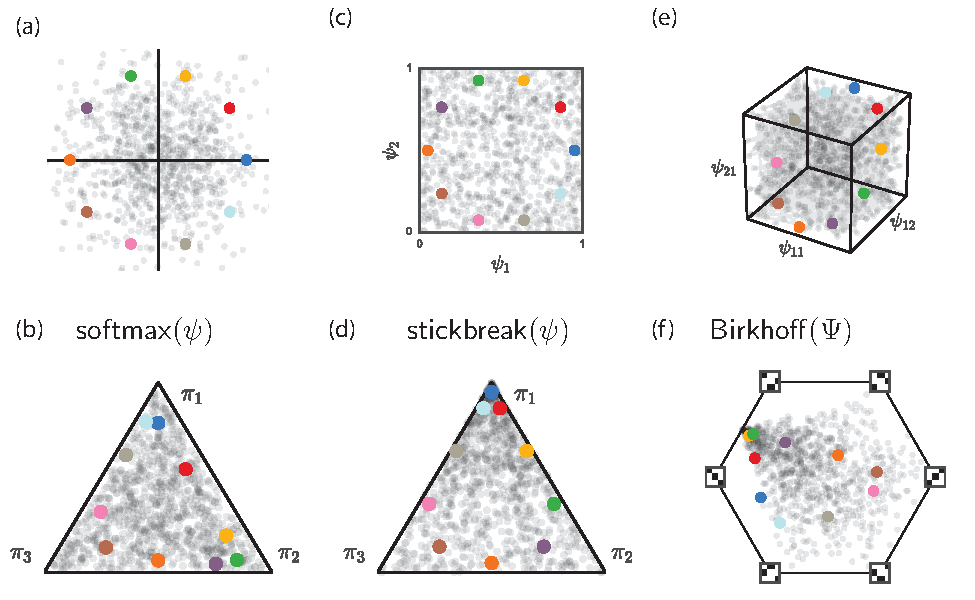
\includegraphics[width=5.in]{../figures/figure1.pdf} 
  \caption{Reparameterizations of discrete polytopes.  (a,b) The
    Gumbel-softmax, or ``Concrete'' transformation maps points
    ${\psi \in \reals^N}$ to points~${x \in \Delta_{N}}$ by adding
    noise and applying the softmax.  Here we show a slice for~$N=3$
    with~$\psi_3=0$. Colored points are aids to visualize the
    transformation.  (c,d) Stick-breaking offers and alternative
    transformation, here from points~$\psi \in [0,1]^{N-1}$ to~$\Delta_N$.
    The ordering of the stick-breaking induces an asymmetry in the
    transformation.  (e,f) We extend this stick-breaking transformation
    to reparameterize the Birkhoff polytope, i.e. the set of doubly
    stochastic matrices. Here,~$\mcB_3$ is reparameterized in terms
    of matrices~$\Psi \in [0,1]^{2 \times 2}$, of which three coordinates
    are shown in (e).  These points are mapped to doubly stochastic
    matrices, which we have projected onto~$\reals^2$ in panel~(f).}
\label{fig:transforms}
\end{figure*}

\subsection{Related Work}
A number of previous works have considered approximate methods of
posterior inference over the space of permutations.

When a point estimate will not suffice, sampling methods like Markov
chain Monte Carlo (MCMC) algorithms may yield a reasonable approximate
posterior for simple problems~\citep{diaconis1988group}.
\citet{harrison2013importance} developed an importance sampling
algorithm that fills in count matrices one row at a time, showing
promising results for matrices with~$O(100)$ rows and columns.  It may
also be possible to turn the Hungarian algorithm into an efficient
sampling algorithms using Perturb-and-MAP \citep{li2013efficient}.
Another line of work considers inference in the spectral domain,
approximating distributions over permutations with the low frequency
Fourier components~\citep{kondor2007multi, huang2009fourier}.  Perhaps
most relevant to this work, \citet{plis2011directional} propose a
continuous relaxation from permutation matrices to points on a
hypersphere, and then use the von Mises-Fisher (vMF) distribution to
model distributions on the sphere's surface. While the vMF
distribution does have a concentration parameter, as the concentration
goes to infinity, the distribution converges to a point on the sphere.
By contrast, we will derive temperature-controlled densities over
points inside or near the Birkhoff polytope such that as the
temperature goes to zero, the distribution converges to an atomic
density on permutation matrices.

\section{Variational permutation inference via reparameterization}
\label{sec:permutation}

Unfortunately, reparameterization-based variational inference  \ref{sub:repa} is not readily available for permutations: as samples  (permutations) are discrete, the function $g$ cannot be continuous. However, recently, there have been a number of proposals to extend the
reparameterization trick to discrete inference problems
via continuous relaxation~\citep{maddison2016concrete,
  jang2016categorical, kusner2016gans}. Essentially, the method is based on replacing the original ELBO objective ~\eqref{eq:elbo} by a surrogate one, arising from replacing the original samples $x$ by a relaxation; that is, now assuming they can belong to a larger, continuous set where derivatives are well defined. This surrogate construction is controlled by a  ``temperature'' knob that dictates the degree of relaxation; how ``far''   is the relaxation from the original discrete problem.
  
These relaxations, however, are not suitable for permutations, as the representation of a permutation as a category requires $N!$ slots. In this section, we develop two relaxations to enable variational permutation inference. In both relaxations the Birkhoff polytope will play a fundamental role, although clear differences exist. Also, in either case we start with a noise distribution $\Xi$ (here, gaussian) and transform it to a ``relaxed" permutation $X$ using a differentiable and invertible mapping $G$, and parameters $\theta$; i.e. $X=G(\Xi;\theta)$. With a suitable choice of priors this is enough to compute all terms of equation \eqref{eq:elbo}. We refer the reader to the supplemental material for details on choice of the (continuous) priors, and on how our assumptions lead to explicit expressions for the ELBO, for both relaxations introduced in the following.
 
\subsection{Stick-breaking transformations of the Birkhoff polytope}
Let~$\Psi$ be an arbitrary matrix in~${[0,1]^{(N-1) \times (N-1)}}$; we will
transform it into a doubly stochastic
matrix,~$X \in [0,1]^{N \times N}$ by filling in entry by entry, starting
in the top left and raster scanning left to right then top to
bottom. Denote the~$(m,n)$-th entries of~$\Psi$ and~$X$ by~$\psi_{mn}$
and~${x}_{mn}$, respectively.

Each row and column has an associated unit-length ``stick'' that we
allot to its entries.  The first entry in the matrix is given by,
$x_{11} = \psi_{11}$.  As we work left to right in the first row, the
remaining stick length decreases as we add new entries. This reflects
the row normalization constraints.  Formally, the stick-breaking
transformation for the first row is given by,
\begin{align*}
  x_{1n} &= \psi_{1n} \left(1 - \sum_{k=1}^{n-1} x_{1k} \right)  & &  \text{for } n=2, \ldots, N-1\\
  x_{1N} &= 1 - \sum_{n=1}^{N-1} x_{1n}.
\end{align*}
However, the remaining rows must now conform to both row- and
column-constraints. That is,
\begin{align*}
x_{mn} &\leq 1- \sum_{k=1}^{n-1} x_{mk} & & \text{(row sum)} \\
x_{mn} &\leq 1- \sum_{k=1}^{m-1} x_{kn} & & \text{(column sum)}.
\end{align*}
Moreover, there is also a lower bound on~$x_{mn}$. This entry must
claim enough of the stick such that what is leftover fits within
the confines imposed by subsequent column sums. That is, each column
sum places an upper bound on the amount that may be attributed to any
subsequent entry. If the remaining stick exceeds the sum of these
upper bounds, the matrix will not be doubly stochastic.  Thus,
\begin{align*}
\underbrace{1 - \sum_{k=1}^n x_{mk}}_{\text{remaining stick}}
  &\leq \underbrace{\sum_{j=n+1}^N (1- \sum_{k=1}^{m-1} x_{kj})}_{
    \text{remaining upper bounds}}.
\end{align*}
Rearranging terms, we have,
\begin{align*}
  x_{mn} &\geq
  % 1- \sum_{k=1}^{n-1} x_{mk} - \sum_{j=n+1}^N (1- \sum_{k=1}^{m-1} x_{kj}) \\
1 - N + n - \sum_{k=1}^{n-1} x_{mk}  +  \sum_{k=1}^{m-1} \sum_{j=n+1}^N x_{kj}.
\end{align*}
Of course, this bound is only relevant if the right hand side is greater than zero.
Taken together, we have~$\ell_{mn} \leq x_{mn} \leq u_{mn}$, where,
\begin{align*}
\ell_{mn} &\triangleq \max \left \{0, \, 1 - N + n - \sum_{k=1}^{n-1} x_{mk}  +  \sum_{k=1}^{m-1} \sum_{j=n+1}^N x_{kj} \right \}
\\
u_{mn} &\triangleq 
\min \left \{1- \sum_{k=1}^{n-1} x_{mk}, \,
1- \sum_{k=1}^{m-1} x_{kn} \right\}.
\end{align*}
Accordingly, we define,~${x_{mn} = \ell_{mn} + \psi_{mn} (u_{mn} - \ell_{mn})}$.
The inverse transformation from~$X$ to $\Psi$ is analogous.
We start by computing~$\psi_{11}$ and then progressively compute
upper and lower bounds and set~${\psi_{mn} = (x_{mn} - \ell_{mn})/(u_{mn} - \ell_{mn})}$.

To complete the reparameterization, we define a parametric,
temperature-controlled density for~$\Psi$.
Let~${\Xi \in \reals^{(N-1) \times (N-1)}}$ be a matrix of standard
Gaussian random variables.  We
define,
\begin{align*}
  \psi_{mn} &= \sigma\left( \frac{\mu_{mn} + \eta_{mn} \Xi_{mn}}{\tau} \right),
\end{align*}
where~${\theta = \{\mu_{mn}, \eta^2_{mn}\}_{m,n=1}^N}$ are the mean
and variance parameters of the
mapping,~${\sigma(u) = (1+e^{-u})^{-1}}$ is the logistic function,
and~$\tau$ is a temperature parameter. As~$\tau \to 0$, the values
of~$\psi_{mn}$ are pushed to either zero or one, depending on whether
the input to the logistic function is negative or positive,
respectively.  As a result, the doubly-stochastic output matrix~$X$ is
pushed toward the extreme points of the Birkhoff polytope, the
permutation matrices.

\subsection{Rounding toward permutation matrices}
\label{sub:rounding}

While relaxing permutations to the Birkhoff polytope is intuitively
appealing, it is not strictly required.  For example, consider the
following procedure for sampling a point \emph{near} the Birkhoff
polytope:
\begin{enumerate}[label=(\roman*)]
\item Input a point~${M \in \reals_+^{N \times N}}$;
\item Project~$M$ onto the Birkhoff polytope (approximately) using the Sinkhorn-Knopp algorithm;
\item Sample a Gaussian random variable~$\Psi$ with mean~$\mathrm{proj}(M)$ and variance~$\Sigma$;
\item Round~$\Psi$ to the nearest permutation matrix,~${P^*(\Psi)}$, using the Hungarian algorithm;
  and
\item Return~${X = \tau \Psi + (1-\tau) P^*(\Psi)}$.
\end{enumerate}
This procedure implicitly defines a distribution over matrices~$X$
parameterized by~$M$ and $\Sigma$, which we will optimize.
Steps (i) and (ii) involve differentiable transformations of
parameter~$M$ to set the mean close to the Birkhoff polytope; the
challenge in computing the density~$p(X; M, \Sigma)$ stems from step
(iv), since the rounding operation is not differentiable.  However,
the rounding output only changes at points that are equidistant from
two or more permutation matrices. In other words, rounding is a
piecewise constant function of~$\Psi$ with discontinuities only at a
set of points with zero measure. In practice, we find that we can
safely ignore these discontinuities.  Furthermore, note
that~${P^*(\Psi) \equiv P^*(X)}$ so that the inverse transformation
is~${\Psi = \tfrac{1}{\tau}X - \tfrac{1-\tau}{\tau} P^*(X)}$.  Taken
together,~$X$ is a linear function of a Gaussian random variable and
its density is,
\begin{align*}
  p(X; M, \Sigma) = \frac{1}{\tau} \distNormal \left( \frac{1}{\tau}X -\frac{1-\tau}{\tau} P^*(X); \, \mathrm{proj}(M), \Sigma \right),
\end{align*}
which is valid for~$X$ in the image of the rounding operation.  In the
zero-temperature limit we recover a discrete distribution on
permutation matrices; otherwise the density concentrates near the
vertices as~${\tau \to 0}$.

Why is step (iii) necessary? Na\"ively, we could sample a matrix and
project it with the Sinkhorn-Knopp algorithm; the problem is that we
could not calculate the resulting density since the Sinkhorn-Knopp
algorithm is non-invertible.  With the algorithm above, Sinkhorn-Knopp
is employed \emph{prior} to sampling, allowing us to compute the
resulting density.

\begin{figure*}[ht] 
   \centering
   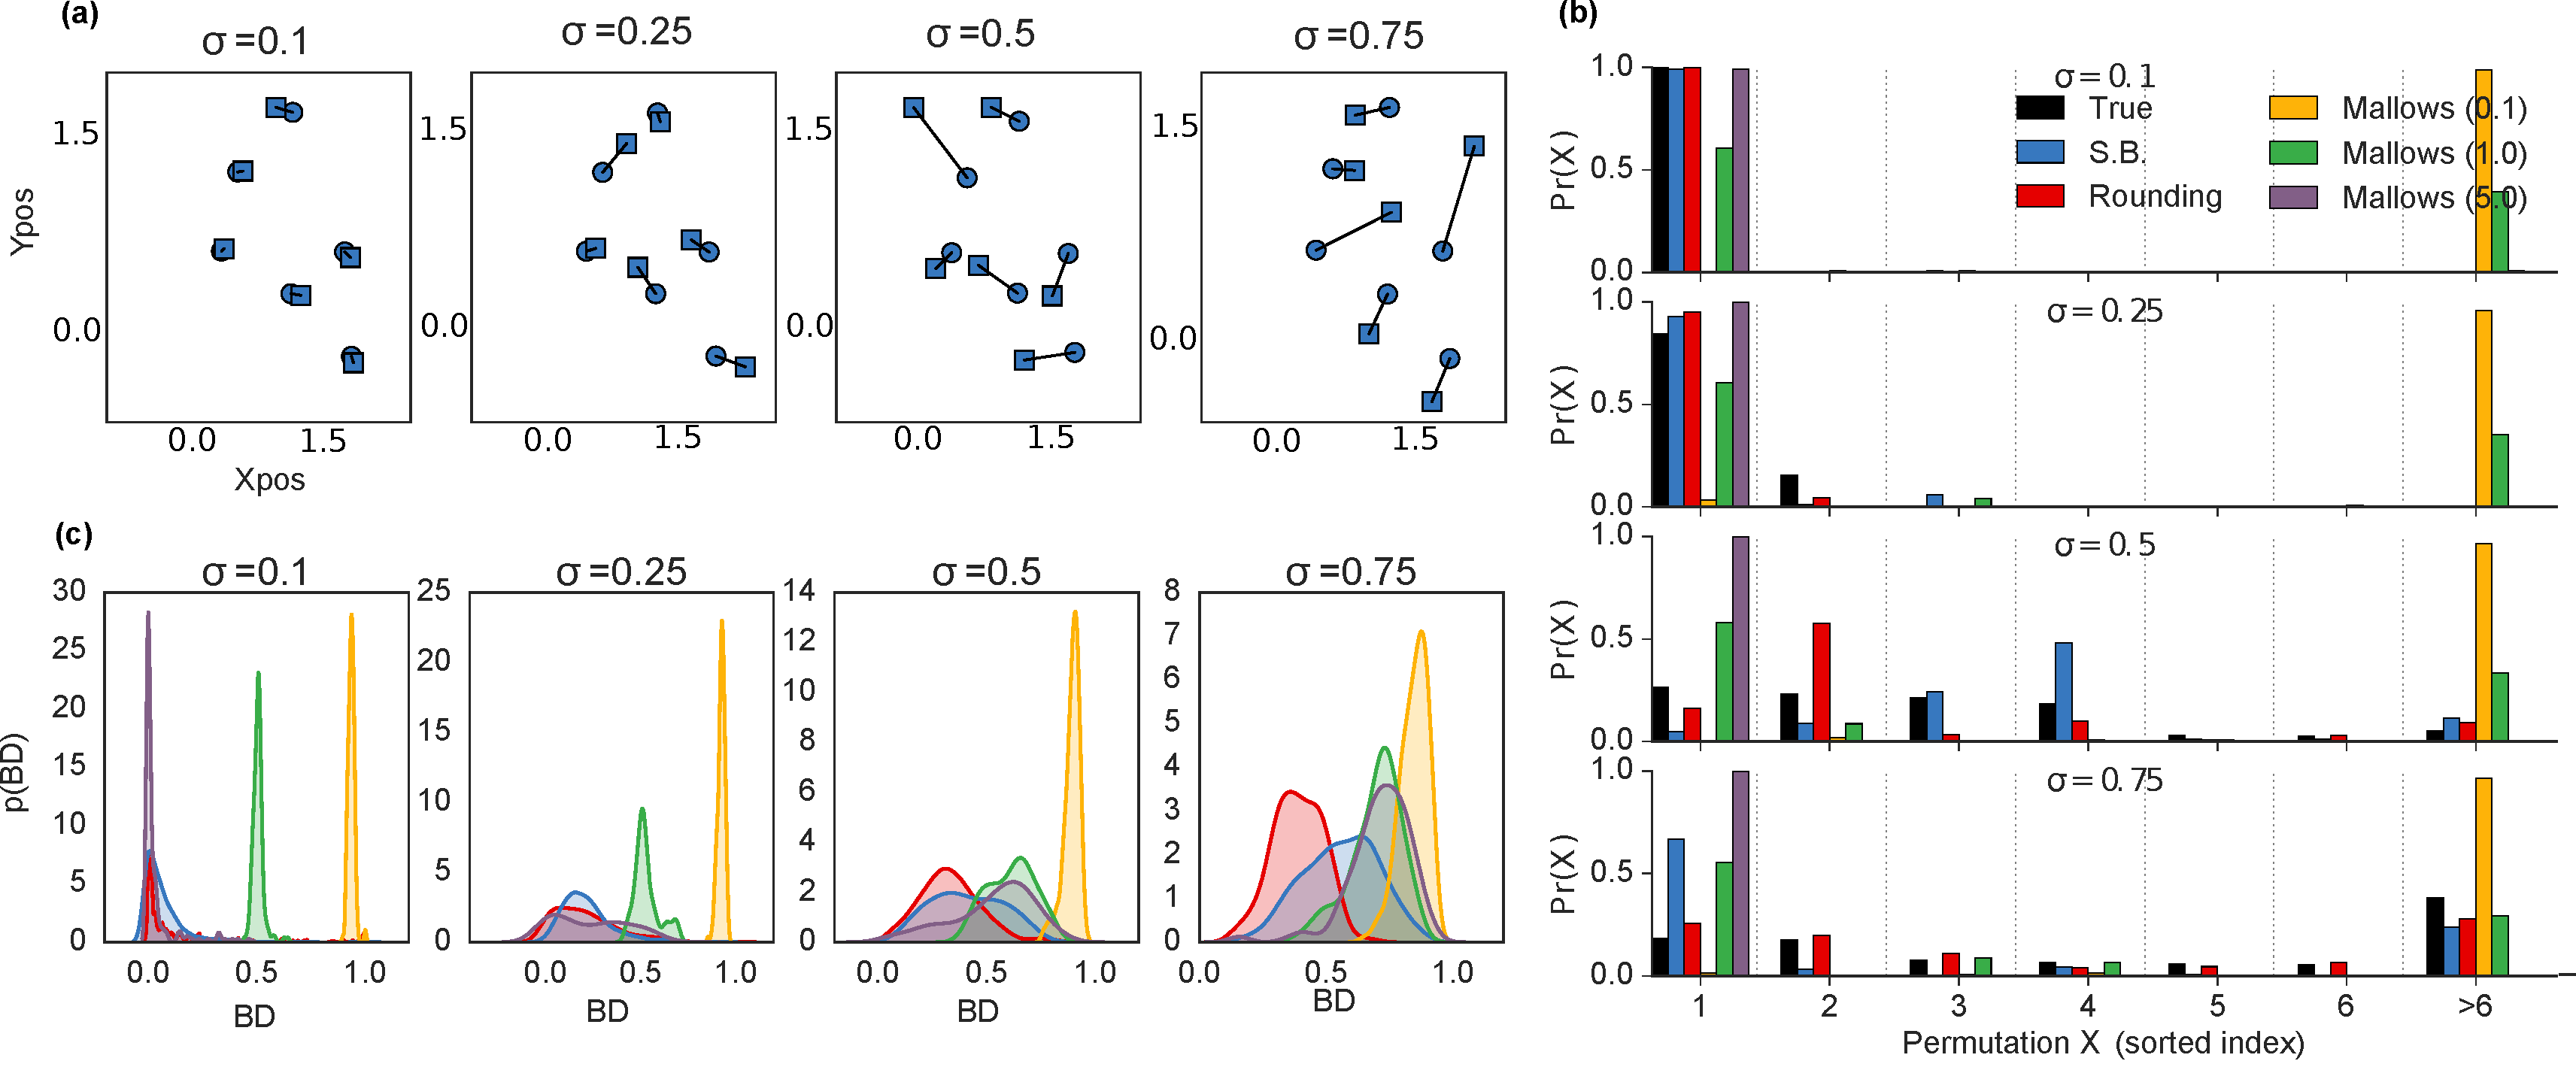
\includegraphics[width=1.0\textwidth]{../figures/figure8.pdf}
   \caption{Synthetic matching experiment results. The goal is to infer the lines that match squares to circles. (a) Examples of center locations (circles) and noisy samples (squares), at different noise variances. (b) For illustration, histograms of the true and inferred posterior distribution of identities along the corresponding BD, for selected cases. Histogram indexes are sorted from the highest to lowest actual posterior probability. Only the 20 most likely configurations are shown, and the 21st bar collapses the mass of all remaining configurations. (c) Population results (histograms) across 200 experiment repetitions of each parameter configuration.}
   \label{fig:synthetic}
\end{figure*}

\subsection{Theoretical considerations}

Stick-breaking and rounding each have their strengths and weaknesses.
Here we list some of their conceptual differences, and in
Section~\ref{sec:synthetic} we evaluate the two approaches
empirically.

\begin{itemize}
\item Stick-breaking relaxes to~$\mcB_N$ whereas rounding relaxes
  to~$\reals^{N \times N}$. The Birkhoff polytope is perhaps
  intuitively nicer, but as long as the log probability accepts
  real-valued matrices, either may suffice.
  
\item Rounding uses the~$O(N^3)$ Hungarian algorithm in its sampling
  process, whereas stick-breaking is a feed-forward,~$O(N^2)$, process.
  \todo{but isn't the Jacobian $O(N^4)$ in both cases?}
  
\item Stick-breaking is a bijective mapping from~$\reals^{(N-1) \times (N-1)}$ to~$\mcB_N$, whereas rounding maps~$\reals^{N \times N}$ to a subset of~$\reals^{N \times N}$.  Consider a simple example of rounding in the one-dimensional simplex, that is, the unit interval.  If~$\tau = 0.5$, the rounding operation maps~$[0,1]$ to~${[0,0.25) \cup [0.75, 1]}$ (the midpoint is arbitrarily rounded up); the resulting density has zero measure in the interval~$[0.25, 0.75)$.  The same is true of rounding toward permutations: the inverse mapping is only defined for points within~$\tau$ of a permutation, and the resulting density is discontinuous at the boundaries. 
  
\item Rounding can easily incorporate constraints.  If certain
  mappings are invalid, e.g.~${X_{mn} \equiv 0}$, they are given an
  infinite cost in the Hungarian algorithm.\footnote{Constraints of
    the form~$X_{m,n} \equiv 1$ simply reduce the dimension of the
    inference problem.}  This is hard to do this with stick breaking
  as it would change the computation of the upper and lower bounds.
  
\item Stick-breaking introduces a dependence on ordering.  While the
  mapping is bijective, a desired distribution on the Birkhoff polytope
  may require a complex distribution for~$\Psi$.  Rounding, by contrast,
  is more ``symmetric'' in this regard.
  
\item Unfortunately, neither admits a simple probability mass function
  on permutations, in contrast to the Gumbel-softmax
  trick~\citep{maddison2016concrete, jang2016categorical}.  This
  complicates the computation of the ELBO, as we discuss next.
\end{itemize}


% First, let us consider an alternative reparameterization of the simplex
% via a stick breaking construction. We break this into two steps. First,
% we transform the noise and parameters to a point in the~${N-1}$ dimensional
% unit hypercube,
% \begin{align}
%   \xi &\sim r(\xi), & 
%   \psi & = f(\theta, \xi),
% \end{align}
% where~${\psi \in [0,1]^{N-1}}$. Then we transform the hypercube to~$\Delta_N$
%   via a stick-breaking transformation,
% \begin{align}
%   x_n = g_n(\psi)
%   &= \begin{cases}
%     \psi_1 & n=1, \\
%     \psi_n \left(1- \sum_{m=1}^{n-1} x_m \right) & 1 < n < N, \\
%     1- \sum_{n=1}^{N-1} x_n & n=N.
%     \end{cases}
% \end{align}
% The intermediate values~$\psi_n$ can seen as the fraction of the
% remaining ``stick'' of probability mass assigned to~${\pi}_n$.  In
% addition to its use in Bayesian nonparametrics, this type of
% transformation has been used in efficient MCMC algorithms for
% multinomial and categorical inference \citep{linderman2015dependent}.

% We focus on standard Gaussian noise~${r(\xi) = \mathcal{N}l(0,I)}$
% and we take~$f$ to be a logistic
% transformation~${\psi_n = \sigma((\mu_n + \eta_n \xi_n) / \tau)}$,
% where ${\sigma(u) = (1+e^{-u})^{-1}}$ is the logistic function
% and~$\tau$ is a \emph{temperature} parameter.  This
% \emph{logistic-normal stick breaking} transformation is parameterized
% by~${\theta = \{\mu_n, \eta_n\}_{n=1}^{N-1}}$, and it enjoys following
% properties: i)~the density of~$x$ can be expressed in closed form as a
% function of~$\mu_n$ and~$\eta_n^2$; ii)~the temperature~$\tau$
% controls how concentrated $p(x)$ is at the vertices of the simplex;
% iii)~with appropriate choices of parameters, in the limit
% ~$\tau \to 0$ we can recover any categorial distribution, i.e., the
% density becomes concentrated on atoms at the~$N$ vertices; and iv)~as
% ~$\tau \to \infty$, the density concentrates on a point in the
% interior of the simplex determined by the parameters. For all
% intermediate temperatures, the density is continuous on the simplex.

% Note that the logistic-normal stick breaking transformation one of
% many available. For example, we could take~$r$ and $f$ to be a
% reparameterization of the Kumaraswamy of beta distributions on the
% unit interval. The former is easily reparameterizable and the
% latter---which leads to the generalized Dirichlet distribution on the
% simplex---can be reparameterized following~\citet{naesseth2017reparameterization}. We include proofs of points (i-iv) and details of the Kumaraswamy and beta stick breaking constructions in the appendix.

% \parhead{Rounding}
% Both the Gumbel-softmax and stick-breaking relaxations consider
% distributions on the simplex, and while this
% offers an intuitive interpretation, it is not strictly required.  For
% example, first consider a distribution on~$\psi \in \reals^N$. These
% points are the rounded to the nearest vertex of the simplex via the
% operator,
% \begin{align}
%   \mathrm{round}(\psi) &= \argmin_{e_n} \| \psi - e_n \|.
% \end{align}
% % This operator partitions~$\reals^N$ into ``Voronoi'' cells
% % centered on the~$N$ vertices,
% % \begin{align}
% %   V_n &=
% %         \left\{\psi \in \reals^N: \, 
% %         \| \psi - e_n \| \leq \| \psi - e_m \| \;
% %         \forall m \in 1, \ldots, N \right\}.
% % \end{align}
% Unfortunately this rounding operator is non-invertible and
% non-differentiable.  Thus, we instead consider a map that pulls a
% point towards its rounded value, by taking a convex combination
% between both. Specifically, we consider the following reparameterization:
% \begin{align}
%   \xi &\sim p(\xi), \\
%   \psi &= f(\theta, \xi), \\
%   x &=  \tau \psi + (1-\tau) \cdot \mathrm{round}(\psi) .
% \end{align}
% In the zero-temperature limit we recover a discrete distribution on
% the vertices. For~$\tau > 0$, the distribution is continuous
% on~$\reals^N$. If the distribution of~$\psi$ is concentrated
% near the simplex---e.g. if~$\theta$ is a point on the simplex
% and~$\xi$ is small, additive Gaussian noise---the rounded points
% will lie close to the simplex as well. Moreover, this technique
% is easily generalized to more complex discrete polytopes. 
% % Moreover, this approach can be generalized to arbitrary discrete we
% % can represent any arbitrary categorical distribution over one-hot
% % vectors. This is shown in the appendix.

\section{Synthetic Experiments}
\label{sec:synthetic}
We are interested in two principal questions: 
 (i) how well can the stick-breaking and rounding re-parameterizations
of the Birkhoff polytope approximate the true posterior distribution
over permutations in tractable, low-dimensional cases? and (ii)
when, if ever, do our proposed continuous relaxations offer
advantages over alternative  Bayesian permutation
inference algorithms?

Before addressing those questions we start by comparing how the categorical counterparts \footnote{That is, simple stick breaking and rounding in the probability simplex.} of our proposed distributions over permutations perform on a simple VAE task.  Results of this task may shed light on the usefulness of our proposed relaxations.

\subsection{Variational Autoencoders (VAE) with categorical latent variables}
We considered the density estimation
task on MNIST digits, as in \cite{maddison2016concrete,
  jang2016categorical}, where observed digits are reconstructed from a
latent discrete code. We used the continuous ELBO for training, and
evaluated performance based on the marginal likelihood, estimated
through the multi-sample variational objective of the discretized
model. We compared against the methods of
\cite{jang2016categorical, maddison2016concrete}, finding similar (although slightly worse) results (Table 1). This difference may be intepreted as the price to be paid in order to enable an extension of a relaxed distribution over categories, to permutations.  In the supplement more results on this task are available.
\begin{table}[t]
  \caption{Summary of results in VAE}
  \label{tab:vae}
  \centering
  \begin{tabular}{ll}
    \textbf{Method} & $- \log p(x)$ \\
    \hline
    Gumbel-Softmax    & 106.7 \\
    Concrete  &  111.5\\
    Rounding &  121.1 \\
    Stick-breaking & 119. 8\\
    \bottomrule
  \end{tabular}
\end{table}


% \begin{table*}[t]
%   \caption{Battacharya distances in the synthetic matching experiment}
%   \label{sample-table}
%   \centering
%   \begin{tabular}{llllllll}
%    & \multicolumn{1}{c}{Rounding} & \multicolumn{1}{c}{Stickbreaking} & \multicolumn{5}{c}{Mallows}\\
%     \cmidrule(lr){2-2} \cmidrule(lr){3-3} \cmidrule(lr){4-8}
%     &    & &   $\theta=0.1$ &  $\theta=1$ & $\theta=2$ & $\theta=5$ & $\theta=10$ \\
%     \midrule
%     $\sigma=0.1$     & .06 & .09  &.93 &.51& .23  & .08 &.08\\
%     $\sigma=0.25$     & .21 & .23 & .92 &.53 & .33&  .27 &.27\\
%      $\sigma=0.5$     & .32 & .41 & .89 &.61 & .53&  .54& .54\\
%      $\sigma=0.75$     & .38   & .55 & .85 &.71 & .69&  .72 &.72\\
   
%     \bottomrule
%   \end{tabular}
% \end{table*}

 \subsection{Synthetic matching experiments}
 To assess the quality of our approximations for distributions over
 permutations, we considered a toy matching problem in which we are given the locations of~$N$ cluster centers and a corresponding set of~$N$
 observations, one for each cluster, corrupted by Gaussian noise.
 Moreover, the observations are permuted so there is no correspondence
 between the order of observations and the order of the cluster centers.
 The goal is to recover the posterior distribution over permutations.
 For~$N=6$, we can explicitly enumerate the~$N!=720$ permutations and
 compute the posterior exactly. 
 
 As a baseline, we consider the Mallows distribution  \cite{Mallows1957} with density over a permutations $\phi$ given by $p_{\theta, \phi_0}(\phi)\propto \exp(-\theta d(\phi,\phi_0))$, where $\phi_0$ is a central permutation, $d$ is a distance between permutations \footnote{Here, $d(\phi,\phi_0)=\sum_{i=1}^N |\phi(i)-\phi_0(i)|$.} and $\theta$ controls the spread around $\phi_0$. This is perhaps the most popular exponential family model for permutations; however, it is too simple and might fail to capture complex features of distributions.

 \begin{table}[h]
  \caption{Mean BDs in the synthetic matching experiment for various methods and observation variances.}
  \label{table:BDs}
  \centering
  \begin{tabular}{lllll}
    & \multicolumn{4}{c}{Variance $\sigma^2$} \\
    \cmidrule(lr){3-4} 
    \textbf{Method} & $.1^2$ & $.25^2$ & $.5^2$ & $.75^2$ \\
    \hline
    Stick-breaking & .09 & .23 & .41 & .55 \\
    Rounding & \textbf{.06} & \textbf{.21}  & \textbf{.32}  & \textbf{.38} \\
    Mallows $(\theta=0.1)$ & .93 & .92 & .89  & .85 \\
    Mallows $(\theta=0.5)$ & .51 & .53  & .61 & .71 \\
    Mallows $(\theta=2)$ & .23 & .33 & .53  & .69 \\
    Mallows $(\theta=5)$ & .08 & .27 & .54 & .72 \\
    Mallows $(\theta=10)$ & .08 & .27 & .54  & .72 \\
    \bottomrule
  \end{tabular}
\end{table}

 Using the Battacharya distance (BD) we measured the discrepancy
 between true posterior and an empirical estimate of the inferred
 posteriors: in our relaxations, by sampling from $q(X; \theta)$ and `rounding'
 to the nearest permutation using the Hungarian algorithm. Likewise, for the Mallows distribution, we set $\phi_0$ to the MAP estimate, also through the Hungarian algorithm, and sampled using MCMC.
 
 We found our method outperforms the simple Mallows distribution, suggesting it might reasonably approximate non-trivial distributions over permutations. Fig ~\ref{fig:synthetic} illustrates our findings by showing sample experiment configurations (a), examples of inferred posteriors (b) and distribution of BD's (c). These histograms are summarized by Table \ref{table:BDs}.


\section{Inferring neuron identities in \textit{C. elegans}}
\label{sec:celegans}

\begin{figure*}[ht]
  \centering
  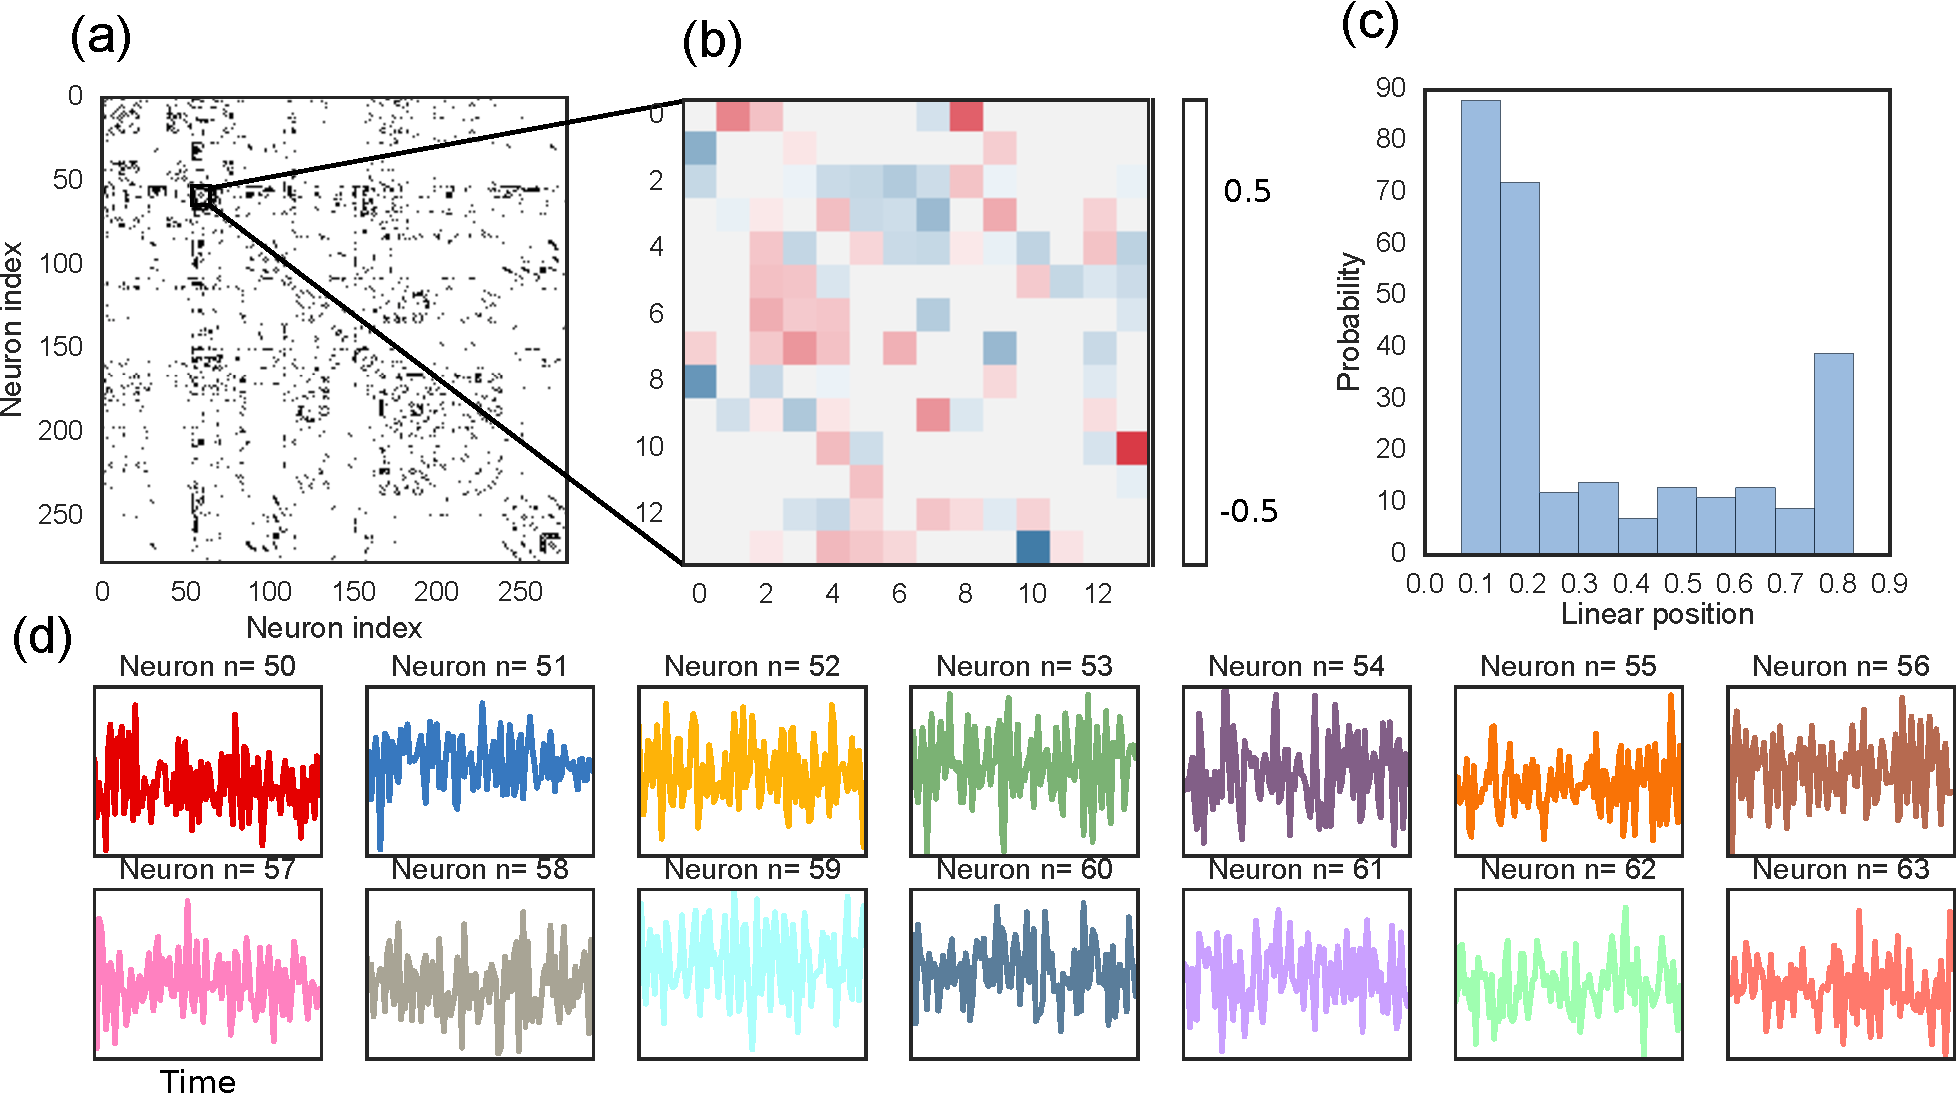
\includegraphics[width=1.0\textwidth]{../figures/figure6.pdf} 
  \caption{Problem setup. (a) Hermaphrodite C.elegans reference
    connectome (from \cite{varshney2011structural,wormatlas})
    consisting of 278 somatic neurons, merging two distinct types of
    synapses: chemical and electrical (gap junctions). (b) Example of
    matrix $W$ consistent with the connectome information (only 14
    neurons for visibility), (c) Distribution of neuron position in
    the body, zero means head and one means tail. From
    \cite{white1986structure,wormatlas} (d). Examples of the dynamical
    system sampled from matrix $W$.}
  \label{fig:connectome}
\end{figure*}

Finally, we consider an application motivated by the study of the neural dynamics in the \textit{Caenorhabditis elegans} (C.elegans)  \cite{Kato2015}, a nematode (worm) of interest for neuroscience, as its neural network changes little from animal to animal. Recent efforts have focused on establishing an accurate and complete neural wiring diagram from anatomical data ~\citep{varshney2011structural} --- a connectome --- that we represent as graph whose nodes are neurons (there are 278 somatic neurons for the hermaphrodyte C. elegans) and whose edges are synapses. Fig ~\ref{fig:connectome}a shows the corresponding adjacency matrix, that we name $\mathcal{C}$.

The C. elegans, then, is particularly suited from investigating how neural activity gives rise to behaviour, a question that has been recently rigorously addressed \cite{Kato2015}. However, there, intensive manual data curation was needed to match neural recordings from calcium imaging techniques to actual neurons. This manual analysis was based on the study of joint patterns of neural activity, and the comparison of observed linear position of recorded neurons to a reference worm. Unfortunately, in some cases, identity could not be exactly resolved, and only putative candidates were inferred. 

This difficulty offers fertile ground for the development of new methods. Recently, promising approaches \cite{Aoki2017} have illustrated the plausibility of using the Brainbow technology \cite{Livet2007} for such purposes, by genetically engineering worms to express fluorescent proteins. 

We prototype an alternative solution that bypasses the need for such sophisticated genetic engineering. Our method embodies the criteria of manual data curation into an algorithm: we resolve neural identity by integrating different sources of information from the connectome, some covariates (e.g. position) and neural dynamics. Moreover, we combine information from many individuals to facilitate identity resolution in hard cases.

\subsection{Probabilistic Model}
We consider $n=1,\ldots, M$ linear (for simplicity) dynamical systems recorded during $t=1,\ldots, T$ time-steps $Y^m_t=P_mWP_m^\top Y^m_{t-1}+\varepsilon_t,\;\varepsilon_t\sim\mathcal{N}(0,I)$ (Fig ~\ref{fig:connectome}d). Each of the $Y_t^m$ is a $N=278$ dimensional vector representing the recorded activity of the entire nervous system. These recordings are a permutation (represented by $P_n$) of the dynamics in a canonical order.  Entries of $W$\footnote{Alternatively, one could have chosen a hierarchical model of $W_m\sim p(W)$, a direction that we avoided here for the sake of simplicity.} are chosen consistently with the connectome: i.e., $W_{i,j}=0$ if $\mathcal{C}_{i,j}=0$. The remaining non-zero entries are then independently sampled from a normal distribution, and scaled by a factor of the spectral radius to ensure stability (see Fig ~\ref{fig:connectome}b for an example of $W$, and see supplement for further details).

We perform variational inference on this model for the joint estimation of the posterior probability of $P_m$ and $W$ given  $Y_m$ \footnote{$\varepsilon$ is assumed known for simplicity, but could otherwise be included in the posterior, or be directly estimated from data.}. For $W$ we use a gaussian prior $p(W)\sim \mathcal{N}(0, I)$. Also, for each of the $P_m$ use the machinery developed in section \ref{sec:permutation}, and we focus on the rounding approximation. 
Then, we approximate the true posterior $p(W,P_m|Y)\propto p(Y|W,P_m)\times p(W)\prod_{m=1}^M p(P_m$)  by a variational family $q$ of the form $q(W,P_m)\equiv q(W)\prod_m^M q(P_m)$, where $q(W)$ is also gaussian and $q(P_m)$ has the distribution described in ~\ref{sub:rounding}. 


\begin{figure*}[ht]
  \centering
  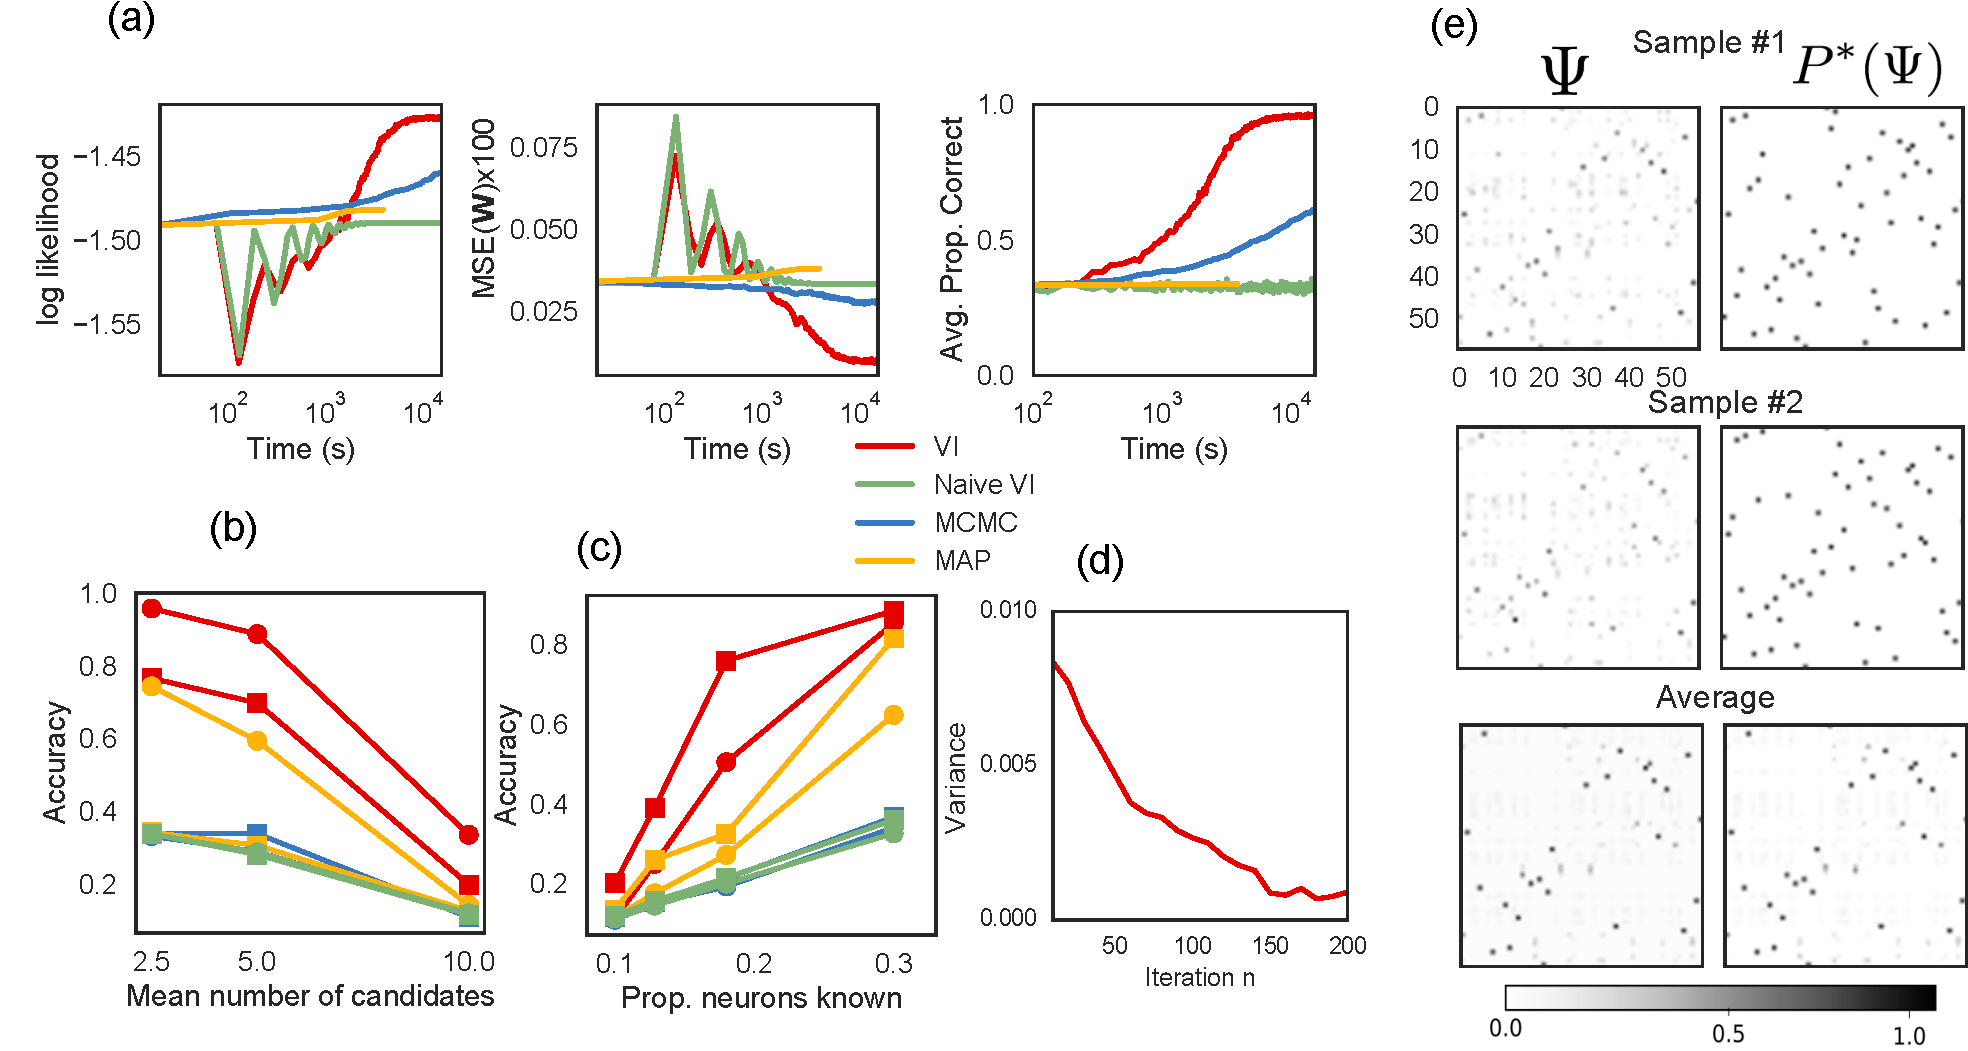
\includegraphics[width=1.0\textwidth]{../figures/figure7.pdf} 
  \caption{Results on the C.elegans inference example. (a) An example of convergence of the algorithm, and the baselines. (b) Accuracy of identity inference as a function of mean number of candidates (correlated with $\nu$), for $M=1$ worm (square) and combining information of $M=5$ worms (circles). (c) Accuracy as a function of the proportion of known networks beforehand,  with $\nu=0.2$ (circles) and $\nu=0.1$ (squares). (d)Variance of distribution over permutations (vectorized) as a function of the number of iterations. (e) Two samples of permutation matrices $P^*(\Psi)$ (right) and their noisy, non-rounded versions $\Psi$ (left) during the execution of the algorithm. The average of many samples is also shown. Presence of grey dots indicate that the sampling procedure is not deterministic.}
\label{fig:elegantresults}
\end{figure*}


Finally, we use neural position along the worm's body to constrain the number of possible neural identities for a given neuron: specifically, we utilize previously documented positions of each neuron as numbers between zero and one \cite{white1986structure,wormatlas} (under the abstraction that a worm can be represented as one-dimensional object, see Fig ~\ref{fig:connectome}c). Then, given reported positions of all (or some) neurons, we can conceive a binary \textit{confusion} matrix $D^m$ so that $D^m_{i,j}=1$ if (observed) neuron $i$ is close enough to (canonical) neuron $j$; i.e., if their distance is smaller than a tolerance $\nu$. We can enforce this constrain during inference, by zeroing corresponding entries in the parameter matrix $M$ described in ~\ref{sub:rounding}.  This modeling choice greatly reduces the number parameters of the model, and facilitates inference. Also, we allow for a certain number of neural identities to be known beforehand, easily encoded in $D^m$ as well.

\subsection{Results}

We compared against three methods: i) naive variational inference, where we don't enforce the constraint that $P$ is a permutation but allow many neurons to be mapped to the same one, ii) MCMC, where one alternates between sampling from the conditionals of $W$ (gaussian) and $P_m$, from which one can sample by proposing local swipes, as described in \cite{Diaconis2009}, and iii) MAP estimator, which can be understood as a `hard' version of ii); instead of iteratively sampling, we alternate between the MAP estimate of $W$ (a ridge regression-like expression) and the MAP of the $P_m$'s. For the $P_m$'s we notice the objective is a quadratic assignment problem (QAP) in $P_m$, that is, it can be expressed as $Trace(APBP^\top)$ for some matrices $A,B$. We used the QAP solver proposed in \cite{Vogelstein2015}. 

As shown in Fig \ref{fig:elegantresults}, our method outperforms each baseline: specifically,  first, Fig \ref{fig:elegantresults}a illustrates convergence to a better solution for a certain parameter configuration. More conclusively, Fig ~\ref{fig:elegantresults}b and  Fig ~\ref{fig:elegantresults}c shows that our method outperforms alternatives when there is much uncertainty on neural position; i.e, when there are many possible candidates (large $\nu$), and where only a small proportion of neurons are known with certitude. Fig ~\ref{fig:elegantresults}c also shows that we indeed obtain benefits from combining information of many worms (although the same applies to MCMC). 

Altogether, these results indicate our method enables a more efficient use of information than MCMC. We interpret this in terms of the observation that in practice variational inference converges faster than MCMC \cite{Blei2017}: we expect MCMC would eventually converge, but in practice it does so slow that asymptotic values are not achieved in reasonable time, as changes in $P$ are very local and proposals (local swipes) are usually rejected. On the other hand, our parameterization allows to more freely sample the parameter space. This is observed in Fig  ~\ref{fig:elegantresults}d: variability of permutation samples is high during iterations (see variability in Fig ~\ref{fig:elegantresults}e), but eventually decays to asymptotic values after more certainty of the true permutation has been accumulated.
\section{Discussion}
Our results provide evidence that permutation variational inference might provide a helpful tool for the inference of neural identity, as it allows to properly represent shared information across animals, and different degrees of certainty based on covariates. In order to apply it to real data it is necessary to consider more realistic models of neural dynamics, which are non-linear but might be well characterized, for example, by a set of atomic low-dimensional linear dynamical systems, each of one corresponding to a certain behavioral state  \cite{Kato2015}. The methodology developed in \cite{Linderman2016} seems particularly suitable to harness that increased level of complexity. \
2.3 3.5 11
\bibliography{refs}
\bibliographystyle{abbrvnat}
\pagebreak 
\appendix
\section*{Supplement}
\subsection*{MNIST reconstructions}
In figure \ref{fig:VAE} we show some MNIST  reconstructions using Gumbel-Softmax, stick-breaking and rounding reparameterizations. In all the three cases reconstructions are reasonably accurate, and there is diversity in reconstructions.
\begin{figure*}[t]
  \centering
  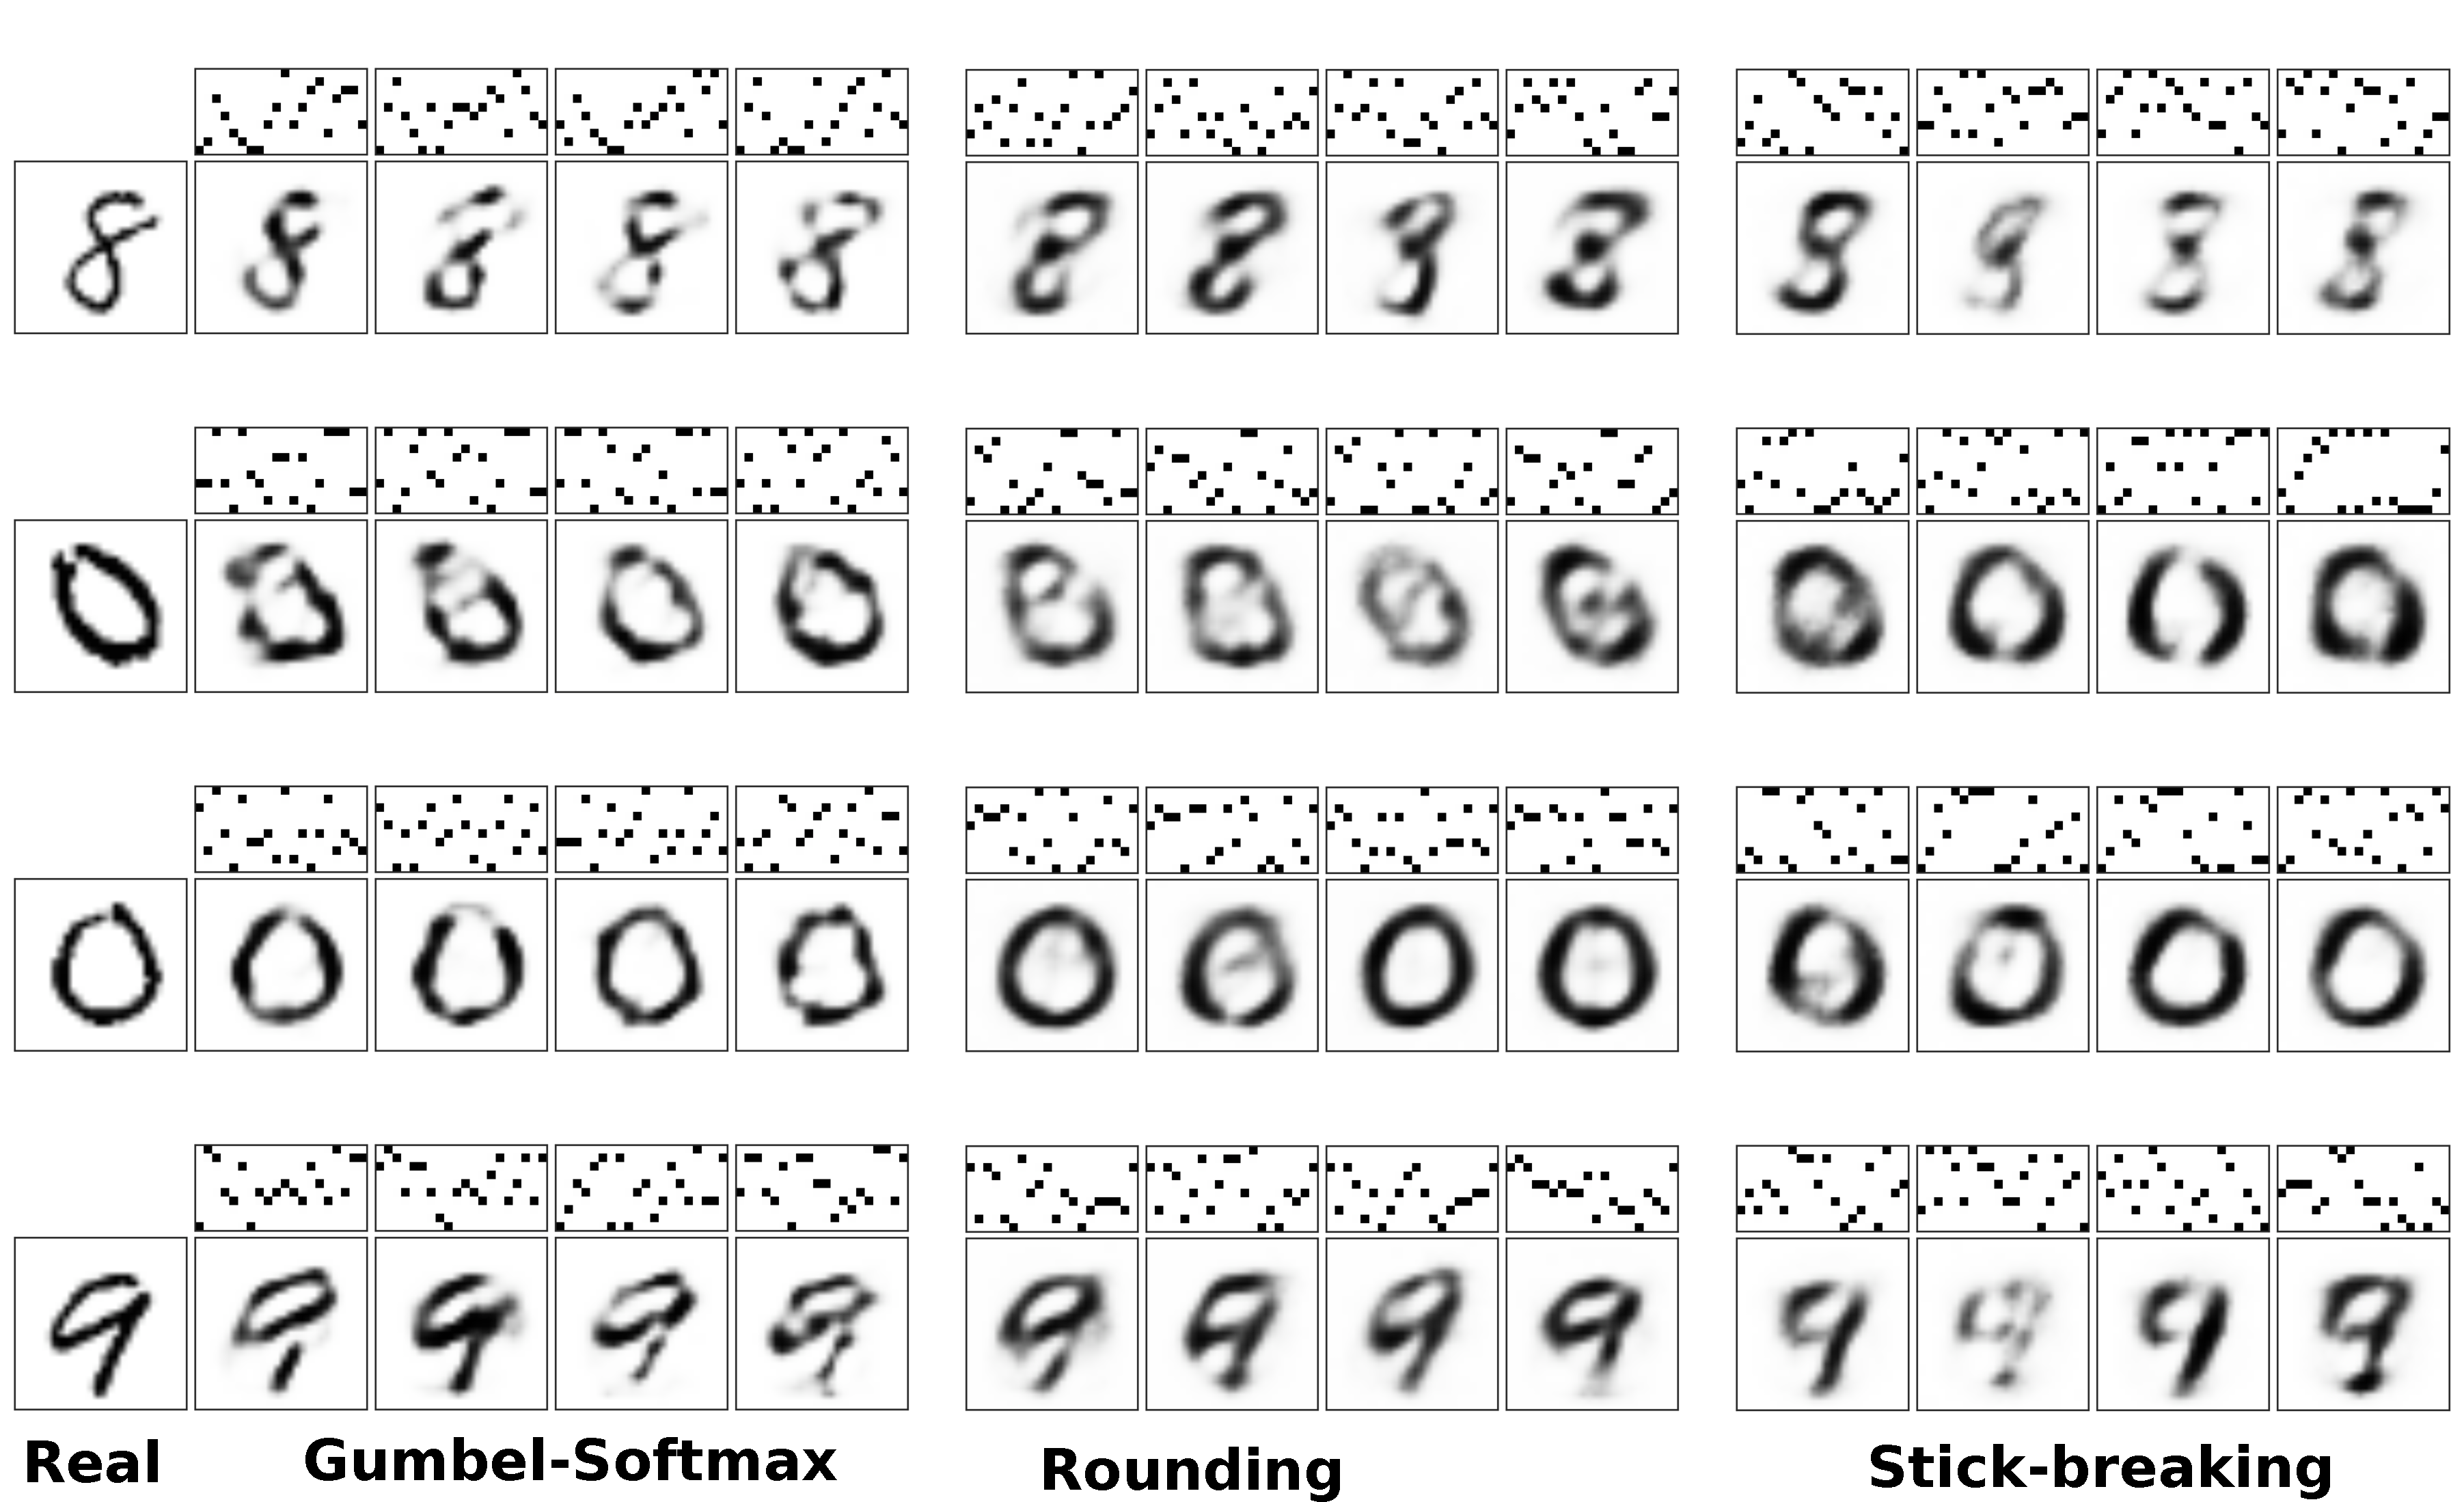
\includegraphics[width=5.in]{../figures/figure4.pdf} 
  \caption{Examples of true and reconstructed digits from their corresponding random codes using with $N=20$ categorical variables with $K=10$ possible values.
  }
\label{fig:VAE}
\end{figure*}

\subsection*{Limit analysis for Stick-breaking}

Here we state and prove that for  the stick-breaking we consider here, we can arrive to either arbitrary points in the i) simplex or ii) to any categorical distribution as limiting cases (in the temperature).  First, we need some lemmas.


\textbf{Lemma 1.}  The following statements are true:
\begin{enumerate} \item the degenerate case where  $z_k$ is deterministic leads to $\pi\sim \delta(\tilde{\pi})$  (i.e, single atom in the point $\tilde{\pi}$). Also, if $z_k$ can be any in $(0,1)$ then any deterministic $\pi$ in the interior of the simplex can be realized.
\item the degenerate case where  $z_k$ are Bernoulli with parameter $p_k(\theta) \in (0,1)$ leads to $\pi$ having an atomic distribution with atoms in the vertices of $\Delta^{k-1}$; i.e, $\pi$ is categorical. We have the following expression for the probabilities of the atoms $\pi_k=1$ (one hot vectors):
\begin{align}
\label{eq:onehotprob}
\nonumber P(\pi_k =1)&= \prod_{i=1}^{k-1} (1-p_i(\theta)) p_k(\theta)  \;\; \ k=2, \ldots, K-1,\\  \nonumber & P(\pi_K =1) = \prod_{i=1}^{K-1} (1-p_i(\theta)).
\end{align}

Moreover, if for each index $k$ any parameter of the Bernoulli variable $z_k$ can be realized through appropriate choice of $\theta$, then any categorical distribution can be realized.

\end{enumerate}
\textit{Proof}: (a) both claims are obvious and come from the invertibility of the function $\mathcal{SB} \circ h (\cdot)$. (b) the formulae for $P(\pi_k =1)$ comes from expressing the event $\pi_k=1$ equivalently as $\pi_k=1,\pi_i=0, i<k$ and then, conditioning backwards successively. The second statement comes from the following expression, which easily follows  from \eqref{eq:onehotprob}:
$$ p_k(\theta)=\frac{P(\pi_k =1)}{P(\pi_{k-1} =1)}\frac{p_{k-1}(\theta)}{1-p_{k-1}(\theta)},\quad k =1,\ldots, K-1.$$
The recursive nature of the above equation gives a recipe to iteratively determine the required $p_k(\theta)$, given  $P(\pi_k =1), P(\pi_{k-1} =1)$ and the already computed $p_{k-1}(\theta)$.


Now we can state our results:

\textbf{Lemma 2.} If $z=\sigma(\psi),\psi\sim\mathcal{N}(\mu,\eta^2)$, then
\begin{enumerate} \item the  limit $\eta\rightarrow 0$ and $\mu$ fixed leads to the deterministic $z=\sigma(\mu)$. 
\item the limit $\mu\rightarrow \infty, \eta^2=\mu/K$ with K constant leads to $z\sim \text{Bernoulli}(\Phi(K))$, with $\Phi(\cdot)$ denoting the standard normal cdf.
\end{enumerate} In both cases the convergence is in distribution 

\textit{Proof}. The first convergence is obvious. To see the second, let's index $\mu_n$ and  study the cdf $F$ of $z_n$ on the interval (0,1) (it evaluates zero below zero and one above one).
\begin{align}F_{z_n}(x)&= P(\sigma(\psi_n)<x) \\
&=P(\psi_n< \sigma^{-1}(x))\\
&=P(\mu_n +\mu_n/K\xi <\sigma^{-1}(x)),\\\
&= P( \xi <\sigma^{-1}(x)K/\mu_n - K)\\
&= \Phi( \sigma^{-1}(x)K/\mu_n - K) 
\end{align}

Therefore, by continuity of $\Phi$ we obtain $F_{\Psi_n}(x)\rightarrow \Phi(-K)$ for all points $x\in(0,1)$. On the other hand, the cdf of a bernoulli random $F$ variable is given by  a step function that abruptly changes at zero, from zero to $1-p$, and at one, from $1-p$ to 1. As convergence occurs at all continuity points (the interval $(0,1)$), we conclude (recall, $1-p= \Phi(-K)\rightarrow \Phi(K)=p$). Notice that the above representation only allows  to converge to $p>0.5$, as $K$ has to be positive. This can be fixed by choosing sequence with negative $\mu$ instead.

\textbf{Proposition.} For the stick-breaking construction, any arbitrary distribution can be realized in the low-temperature limit. Also, in the high-temperature limit convergence is to certain point(s) in the interior of the simplex.

\textit{Proof}: Consider each distribution separately

We have $z_k = \sigma\left( \frac{\mu_k+\eta_k\xi}{\tau}\right)$, in the low temperature case use Lemma 2 (b) by the always available representation  $K= \frac{\mu}{\eta^2}$and conclude by Lemma 1(b). In the high temperature case convergence is to the point $\pi = \mathcal{SB}(0.5,0.5,\ldots, 0.5)$.


%\subsection{Rounding}
%Here we have two extremes: at $\tau =1$ we obtain a continuous distribution in the space (here, gaussian). If $\tau=0$ the resulting distribution has only atoms in the one-hot vectors $p_n$, in this proof assumed to be the one-hot vectors. We show that in this case it is possible to represent any arbitrary categorical distribution through a judicious choice of the parameters.


%\textbf{Proposition:} In the zero temperature case, i.e., $\pi  = R^\mathcal{P}(\psi)$ it is possible to represent any arbitrary distribution i.e, for any $\alpha$ in the $N-1$ simplex there exists gaussian parameters $(\mu, \eta)$ so that   $P(\pi = p_n)  = \alpha_n$. Points inside the simplex are realized directly, while distributions with some $\alpha_k=0$ are realized through a limiting process in the parameters.

%\textit{Proof:} First set $\eta_n=1$. By representing $\psi = \mu + \xi$ where $\xi\sim\distNormal(0, I)$ we see that
%$$\alpha_n = P(R^\mathcal{P}(\mu + \xi) = p_n ) = P(\mu + \xi \in V^\mathcal{P}_{n}) = P(\xi \in V^\mathcal{P}_{n} - \mu) =  \int_{V^\mathcal{P}_{n} - \mu} \frac{1}{(2\pi)^\frac{N}{2}}e^{-\frac{||x||^2}{2}} dx.$$
%Three conclusions are drawn from the above: first, we see that probabilities are ultimately gaussian integrals over a new partition, a translation of the Voronoi regions $V^\mathcal{P}_{n}$. Second,
%the map $(\mu_1,\ldots,  \mu_n)\xrightarrow{m} (\alpha_1,\ldots, \alpha_n)$ is continuous by virtue of the dominated convergence theorem \cite{browder2012mathematical}: indeed, if $\mu_i\rightarrow \mu$ then $(\alpha^i_1,\ldots, \alpha^i_n) \rightarrow (\alpha_1,\ldots, \alpha_n)$, as the $\alpha^i_n$ are integrals that can be expressed using indicator functions in the integrands (which are all bounded by the integrable gaussian density), and as pointwise convergence of the indicators holds because of the continuity of the translation operator $f_\mu(\cdot) = \cdot + \mu$. Third, for each $q\in(0,1)$ it is possible to choose $\mu$ so that $\alpha_n =q$ and $\alpha_m = (1-q)/(n-1)$. Indeed, by moving $\mu_n$ between $-\infty$ and $\infty$ while keeping the other $\mu_k$ fixed then $V^\mathcal{P}_{n} - \mu$ fluctuates between the empty set ($\alpha_n =0$) and the entire space ($\alpha_n=1$). Therefore, by the continuity of $m$ and the intermediate value theorem, every value in $\alpha_n\in (0,1)$ is realized, and by symmetry the other $\alpha_k$ occupy the remaining mass uniformly. 

%To conclude, we use the fact that the image of a convex set through a continuous function is also convex \cite{Rockafellar70}. We also showed that for each tolerance $\epsilon$ the image of $m$ contains these $\epsilon$-one-hot vectors: that is, the points with $(1-\epsilon)$ in one coordinate and $\epsilon/ (n-1)$ in the rest. Then, given a point in the interior of the simplex choose $\epsilon$ small enough so it is in the convex hull of the $\epsilon$-one vectors. Then, by the above theorem there must be a pre-image $\mu$ that realizes this point.

%For $\alpha$ with zero entries the above arguments has to be extended to permit a limit process where $\mu$ goes to either infinity or infinity. It is easy to see that by that extension it is possible to represent any $\alpha$ in the border of the simplex.


\subsection*{Variational inference for Permutation details}

\subsection*{Continuous prior distributions.} 
Continuous relaxations requires
re-thinking of the objective. As in \cite{maddison2016concrete}, we
maximize a relaxed ELBO, for which we need to specify a new continuous
prior $p(x)$ over the latent variables. Moreover, it is critical to conceive sensible priors for permutations, that could serve in a variational inference routine to penalize configurations that are away from permutation matrices (i.e. close to the barycenter of the Brikhoff polytope).

For our categorical experiment on MNIST we use a mixture of Gaussians around
each vertex,~${p(x) = \tfrac{1}{N} \sum_{n=1}^N \mathcal{N}(x \given e_k, \eta^2)}$. 
This can be extended to permutations, where use a mixture of Gaussians for each
dimension,
\begin{align}
\label{eq:permprior}
  \nonumber p(X) &= \prod_{m=1}^N \prod_{n=1}^N
  \frac{1}{2} \left(\mathcal{N}(x_{mn} \given 0, \eta^2) + \distNormal(x_{mn} \given 1, \eta^2 \right).
  \end{align}
Although this prior puts significant mass invalid points
(e.g.~$\bone$), it penalizes $X$ that far from~$\mcB_N$.

\subsection*{Deriving an expression for the ELBO}
Here we show that if $X=G(\Xi;\theta)$ with $G$ differentiable one can evaluate the second term in equation \eqref{eq:elbo} \footnote{Notice that we uppercase the variables in \eqref{eq:elbo} this is in consistency to our notation in section \ref{sec:permutation}}. Moreover, here, to exploit the similarities between both methods (stick-breaking and rounding), we further factor $G$ into two functions: $G=H \circ F$, $X = H(\Psi)$ and $\Psi = F(\Xi; \theta)$ (both $H,F$ invertibles). This means all dependency of $X$ in the parameters is through $\Psi$. Under this assumption, and denoting $\Psi\sim p(\Psi,\theta)$, the second term in equation \eqref{eq:elbo} (without gradient) can be computed as:
 then \begin{align} \nonumber
\E_{r(\Xi)} \left[- \log q(G(\Xi;\theta)); \theta) \right] = & \bbH(\Psi; \theta) +\\ \nonumber & E_{r(\Xi)}\left[\log | DH(F(\Xi,\theta))|\right].\end{align}
\textbf{Proof}:
Indeed, first, it is obvious that $$\E_{r(\Xi)} \left[- \log q(G(\Xi;\theta)); \theta) \right] = \E_{r(\Xi)} \left[- \log q(H(F(\Xi,\theta)); \theta) \right] $$
Then, by the `Law of the Unconscious Statistician' we have:
 $$\E_{r(\Xi)} \left[- \log q(H(F(\Xi,\theta)); \theta) \right] = \E_{p(\Psi;\theta)} \left[- \log q(H(\psi); \theta) \right]. $$
Now, by the change of variable theorem and derivative and determinant inversion rules, we obtain ($D$ means the Jacobian, the matrix of derivatives) :\begin{align}
\nonumber q(H(\Psi); \theta) & = p(H^{-1}(X) ;\theta)  |DH ^{-1}(X) | \\ \nonumber
 & = p(\Psi; \theta) | DH (\Psi) | ^{-1}.
 \end{align}
 To conclude we use once more the Law of the Unconscious Statistician:
 \begin{eqnarray}
\nonumber \E_{r(\Xi)} \left[- \log q(G(\Xi;\theta)); \theta) \right]  &= \E_{p(\Psi;\theta)}\left[ - \log p(\Psi;\theta)\right] +   \\ & \nonumber \E_{p(\psi;\theta)}\left[\log | DH(\psi)|\right] \\ \label{eq:elbo2} 
 &= \bbH(\Psi; \theta)+ \\ \nonumber & E_{r(\xi)}\left[\log | DH(F(\Xi;\theta))|\right].\end{eqnarray}
 

\subsection*{Estimating the ELBO} 
Here we describe how to compute each of terms of equation \eqref{eq:elbo2}, needed for ELBO computations. First, as $\Psi$ is gaussian for both rounding and stick-breaking, the entropy term is straightforward and equal to $N\log(\eta^2 2\pi e )/2$ ($\eta$ may depend on the temperature and depends on the method). 

Notice that to state $\Psi$ is gaussian in the stick-breaking case we slightly deviate from \ref{sec:permutation}. Specifically, here we call $\Psi=\frac{\mu_{mn} + \eta_{mn} \Xi_{mn}}{\tau} $ and define $\Psi' = \sigma(\Psi)$.

The second term of equation \eqref{eq:elbo2} is estimated using Monte-Carlo samples, and its derivation depends on the method. 

\subsubsection*{Rounding}
Here 
 $H$ is piecewise linear: the set of discontinuities (border of the 'Voronoi cells' associated to each permutation) has Lebesgue measure zero. So we can still apply the change of variables theorem. Therefore, 
$\log |DH(F(\Xi;\theta)) |= N\log
\tau$. This means we don't even need to take samples to compute this term.


\subsubsection*{Stick-breaking}

It is important to note that the transformation $H$ that maps $\Psi'\rightarrow X$ is only piecewise
continuous: the function is not differentiable at the points where
the bounds change; for example, when changing~$\Psi'$ causes the
active upper bound to switch from the row to the column constraint
or vice versa.  

Notice that these bounds only depend on values of~$X$ that
have already been computed; i.e., those that are above or to the left of
the~$(i,j)$-th entry. Thus, the transformation from ~$\Psi'$ to~$X$
is feed-forward according to this ordering.  Consequently, the
Jacobian of the inverse transformation $H^{-1}$ ,~$\mathrm{d}\Psi' / \mathrm{d} X$,
is lower triangular, and its determinant is the product of its diagonal,
\begin{align}
\nonumber \left| \frac{\mathrm{d} \Psi'} {\mathrm{d} X} \right|
&= \prod_{i=1}^{n-1} \prod_{j=1}^{n-1} \frac{\partial \psi_{ij} }{\partial {\pi}_{ij}} \\
\nonumber &= \prod_{i=1}^{n-1} \prod_{j=1}^{n-1} \frac{\partial}{\partial {\pi}_{ij}}
\sigma^{-1} \left( \frac{{\pi}_{ij} - \ell_{ij}}{u_{ij} - \ell_{ij}} \right ) \\
\nonumber &= \prod_{i=1}^{n-1} \prod_{j=1}^{n-1}
\left( \frac{1}{u_{ij} - \ell_{ij}} \right )
\left( \frac{u_{ij} - \ell_{ij}}{{\pi}_{ij} - \ell_{ij}} \right )
\left( \frac{u_{ij} - \ell_{ij}}{u_{ij} - {\pi}_{ij}} \right ) \\
\nonumber &= \prod_{i=1}^{n-1} \prod_{j=1}^{n-1}
\frac{u_{ij} - \ell_{ij}}{({\pi}_{ij} - \ell_{ij}) (u_{ij} - {\pi}_{ij})}
\end{align}

To compute the gradient of the forward transformation $H$ one simply needs to invert the above (or put a negative sign, in the logarithm scale). Finally,  to incorporate the effect of $\sigma$ ($\Psi'=\sigma(\Psi)$, by the chain rule,  one only needs to add a term corresponding to this derivative, $d\sigma(x)/dx=\sigma(x)\sigma(-x)$. 
\end{document}
